\documentclass[10pt,a4paper]{article}
\usepackage[utf8x]{inputenc}
\usepackage{ucs}
\usepackage[left=2.00cm, right=2.00cm, top=2.00cm, bottom=2.00cm]{geometry}
\renewcommand\familydefault{\sfdefault}

\title{Robotics - WS1819}
\author{}
\date{2018}

%math
\usepackage{amsmath}
\usepackage{amsfonts}
\usepackage{amssymb}
\usepackage{amstext}
\usepackage{mathtools}

%graphics
\usepackage{graphicx}
\usepackage{floatflt}
\usepackage{float}

%tabular
\usepackage{tabularx}
\usepackage[font=small,labelfont=small]{caption}
\usepackage{colortbl}
\usepackage[dvipsnames]{xcolor}
%\renewcommand{\arraystretch}{2}
%\arrayrulecolor{white}

%tikz
\usepackage{tikz}
\usetikzlibrary{shapes, petri}
\tikzstyle{ell}=[ellipse,draw, yshift=-2mm]
\tikzstyle{rec} = [rectangle, draw]
\tikzstyle{dia} = [diamond, aspect=2, draw, yshift=-5mm]
\tikzstyle{cir} = [circle, draw, minimum size=3mm]
\tikzstyle{arrHV} = [to path={-| (\tikztotarget)}]
\tikzstyle{arrVH} = [to path={|- (\tikztotarget)}]
\tikzstyle{whileright} = [xshift=20mm, yshift=-3mm]
\tikzstyle{whileleft} = [xshift=-20mm, yshift=-3mm]
\tikzstyle{txtright} = [above, xshift=15mm]
\tikzstyle{txtleft} = [above, xshift=-15mm]
\tikzstyle{empty} = [coordinate]
\usetikzlibrary{positioning}

%listings
\usepackage{listings}
\lstdefinestyle{costum} {
	language=Bash,
	basicstyle=\footnotesize\ttfamily,
	keywordstyle=\bfseries\color{cyan!50!blue},
	commentstyle=\itshape\color{black!50},
	%identifierstyle=\color{blue},
	stringstyle=\color{green!50!black},
	morekeywords={returns, loop, each}
}
\lstset{style=costum}


%costum layout
\setlength{\parindent}{0cm}
\usepackage{fancyhdr}
\usepackage{xcolor}
\pagestyle{fancy}
\fancyhf{}
\fancyhead[L]{
	\strut\rlap{\color{orange!50!black}\rule[-\dp\strutbox]{\headwidth}{\headheight}}
	\textcolor {white} {Summary: Robotics}}
\fancyfoot[L]{
	\strut\rlap{\color{orange!50!black}\rule[-\dp\strutbox]{\headwidth}{\headheight}}
	\textcolor {white} {last changed: \today}}
\fancyhead[R]{\textcolor{white}{Winter semester 2018/19}}
%\lfoot{}
\fancyfoot[R]{\textcolor{white} {\thepage}}
%\renewcommand{\footrulewidth}{1pt}

%multicol
\usepackage{multicol}
%\setlength{\columnseprule}{0pt}
%\setlength{\columnsep}{20.0pt}



%custom title color
\usepackage{titlesec}
%\titleformat{\section}
%{\color{cyan!80!blue}\normalfont\Large\bfseries}
%{\color{black}\thesection}{1em}{}

%\titleformat{\subsubsection}
%{\color{blue!30!black!70}\normalfont\bfseries}
%{\color{black}\thesection}{1em}{}

\setcounter{secnumdepth}{4}

%\titleformat{\paragraph}
%{\color{green!30!black!70}\normalfont\normalsize\bfseries}{\theparagraph}{1em}{}
%\titlespacing*{\paragraph}
%{0pt}{3.25ex plus 1ex minus .2ex}{1.5ex plus .2ex}

%tab
\newcommand{\tab}[1][1]{\hspace*{#1cm}}

%color_summary
\newcommand{\sumcolor}[1]{\textcolor{red!10!green!40!blue}{#1}}

%coloring
\newcommand{\redr}{\textcolor{red}{r}}
\newcommand{\greeng}{\textcolor{green}{g}}
\newcommand{\blueb}{\textcolor{blue}{b}}

%other
\usepackage{enumerate}

%hyperref
\usepackage{hyperref}

%vector
\newcommand{\vect}[1]{\ensuremath{\begin{bmatrix}#1\end{bmatrix}}}

%other
\newcommand{\atan}{\ensuremath{\mathrm{atan2 }}}


%Geprüft:
%Coordinate Frames
%Forward Kinematics
%Inverse Kinematics
%Jacobians
%Dynamics
%Trajectories
%Manipulator-mechanics design
%Linear Control
%Nonlinear Control
%Force control

%TODO
%rotation about x, y and z expressed by rotation matrices


\begin{document}
\tableofcontents
\newpage

\section{Coordinate Frames}

\subsection{Descriptions}
\begin{itemize}
	\item used to specify attributes of various objects with which the manipulation system deals (parts, tools, manipulator)
\end{itemize}

\subsubsection{Description of a position}
Let $A$ be a defined coordinate system in addition to the universe coordinate system and $P$ a position vector. Then \\
\begin{equation*}
^AP = \vect{p_x \\ p_y \\ p_z} \\
\end{equation*}
is a point represented as a vector in the coordinate system $\{A\}$ ($p_x$, $p_y$ and $p_z$ indicate distances along the axes of $\{A\}$)

\begin{figure}[H]
	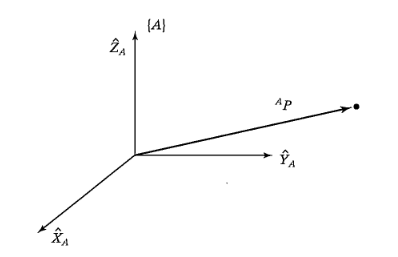
\includegraphics[width=0.5\columnwidth]{imgs/position}
\end{figure}


\subsubsection{Description of an orientation}
\begin{itemize}
	\item Is a description of a coordinate system relative to the reference system
\end{itemize}

Let $\{B\}$ be a coordinate system and \\
the unit vectors giving the principal direction of the coordinate system $\{B\}$ be: $\hat{X}_B$, $\hat{Y}_B$, $\hat{Z}_B$ and \\
let $\{A\}$ be a coordinate system (reference coordinate system). The unit vectors giving the principal direction of $\{B\}$ relative to $\{A\}$ are: \\
\begin{equation*}
^A\hat{X}_B, ^A\hat{Y}_B \text{ and } ^A\hat{Z}_B
\end{equation*}
The rotation matrix which describes $\{B\}$ relative to $\{A\}$ is defined as:
\begin{equation*}
_B^AR := \vect{^A\hat{X}_B & ^A\hat{Y}_B & ^A\hat{Z}_B} = \begin{bmatrix}
r_{11} & r_{12} & r_{13} \\
r_{21} & r_{22} & r_{23} \\
r_{31} & r_{32} & r_{33} \\
\end{bmatrix} = \begin{bmatrix}
\hat{X}_B ⋅ \hat{X}_A & \hat{Y}_B ⋅ \hat{X}_A & \hat{Z}_B ⋅ \hat{X}_A \\
\hat{X}_B ⋅ \hat{Y}_A & \hat{Y}_B ⋅ \hat{Y}_A & \hat{Z}_B ⋅ \hat{Y}_A \\
\hat{X}_B ⋅ \hat{Z}_A & \hat{Y}_B ⋅ \hat{Z}_A & \hat{Z}_B ⋅ \hat{Z}_A \\
\end{bmatrix} = \vect{^B\hat{X}^T_A \\ ^B\hat{Y}^T_A \\ ^B\hat{Z}^T_A} = ~^A_BR^T
\end{equation*}

\paragraph{Inverse of Rotation matrix}
\begin{equation*}
^A_BR = ~^B_AR^T = ~^B_AR^{-1}
\end{equation*}

\subsubsection{Description of a frame}
\begin{itemize}
	\item is a set of four vectors giving position and orientation information
	\item is a coordinate system with a position vector which locates its origin relative to some other embedding frame
\end{itemize}

Let $\{A\}$ be a coordinate system. The frame $\{B\}$ is defined as
\begin{equation*}
\{B\} := \{~^A_BR, ~^AP_{BORG}\}
\end{equation*}
where $^A_BR$ is a rotation matrix and $^AP_{BORG}$ is the vector that locates the origin of the frame $\{B\}$

\begin{figure}[H]
	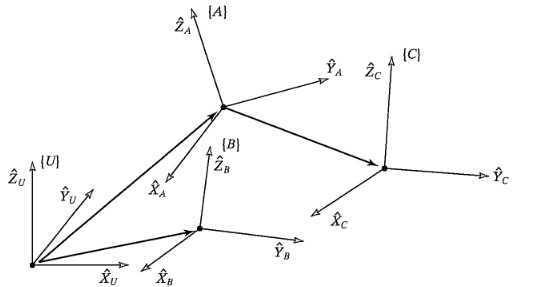
\includegraphics[width=0.5\columnwidth]{imgs/frames}
\end{figure}

\subsection{Mappings}
\begin{itemize}
	\item Changing descriptions from frame to frame
\end{itemize}
\subsubsection{Mappings involving translated frames}
Let $\{A\}$ and $\{B\}$ be frames with the same orientation. \\
Let $^AP_{BORG}$ be a vector that locates the origin of $\{B\}$ relative to $\{A\}$ \\
and $^BP$ a vector that locates a point P relative to $\{B\}$. \\
Then this point relative to $\{A\}$ is defined as:
\begin{equation*}
^AP := ~^BP + ~^AP_{BORG}
\end{equation*}

\begin{figure}[H]
	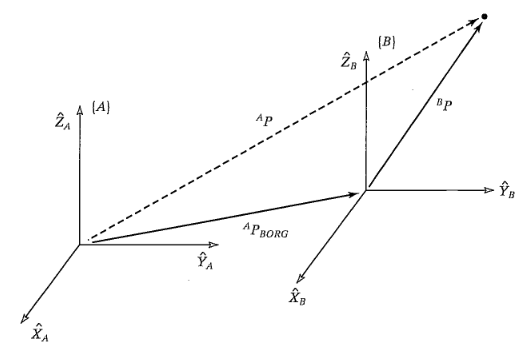
\includegraphics[width=0.5\columnwidth]{imgs/translation}
\end{figure}

\subsubsection{Mappings involving rotated frames}
Let $\{A\}$ and $\{B\}$ be frames with the same origin and \\
$^A_BR$ a rotation matrix that describes $\{B\}$ relative to $\{A\}$. \\
Let $^BP$ be a vector that locates a point P relative to $\{B\}$. \\
Then this point relative to $\{A\}$ is defined as:
\begin{equation*}
^AP := ~^A_BR ⋅ ~^BP
\end{equation*}

\begin{figure}[H]
	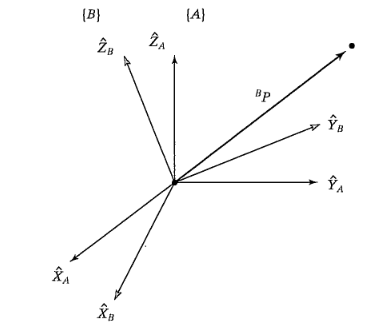
\includegraphics[width=0.5\columnwidth]{imgs/rotation}
\end{figure}

\subsubsection{Mappings involving general frames}
Let $\{A\}$ and $\{B\}$ be frames and\\
$^A_BR$ a rotation matrix that describes $\{B\}$ relative to $\{A\}$. \\
Let $^AP_{BORG}$ be a vector that locates the origin of $\{B\}$ relative to $\{A\}$. \\
Let $^BP$ be a vector that locates a point P relative to $\{B\}$. \\
Then this point relative to $\{A\}$ is defined as:
\begin{equation*}
^AP := ~^A_BR ⋅ ~^BP + ~^AP_{BORG}
\end{equation*}
\begin{equation*}
\vect{^AP \\ 1} = \left[\begin{array}{c|c}
^A_BR & ^AP_{BORG} \\ \hline 0~ 0~ 0 & 1
\end{array}\right] ⋅ \vect{^BP \\ 1}
\end{equation*}
\begin{equation*}
	^AP =~ ^A_BT ⋅~^BP
\end{equation*}
where $\vect{^AP \\ 1}$ is a $4 \times 1$ position vector and the $4 \times 4$ matrix is called a homogeneous transform

\begin{figure}[H]
	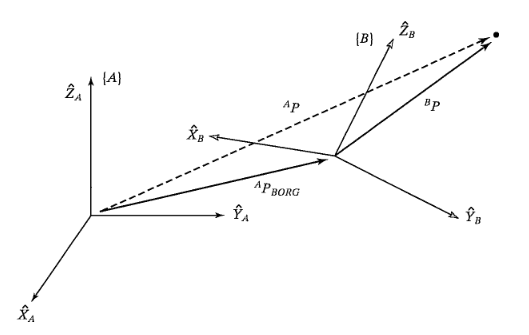
\includegraphics[width=0.5\columnwidth]{imgs/mapping}
\end{figure}

\subsection{Operators}
\subsubsection{Translational operators}
Let $^AP_1$ be a vector that is translated by a vector $^AQ$. \\
The result of the operation is a new vector $^AP_2$ calculated as:
$$
	^AP_2 = ^AP_1 + ^AQ
$$
$$
	^AP_2 = D_Q(q) ⋅~^AP_1
$$
where $D_Q(q) = \begin{bmatrix}
	1 & 0 & 0 & q_x \\
	0 & 1 & 0 & q_y \\
	0 & 0 & 1 & q_z \\
	0 & 0 & 0 & 1
\end{bmatrix}$ and $q_x$, $q_y$ and $q_z$ are the components of the translation vector $Q$ and $q = \sqrt{q_x^2 + q_y^2 + q_z^2}$

\begin{figure}[H]
	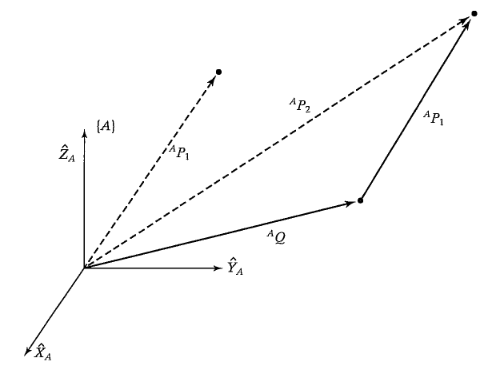
\includegraphics[width=0.5\columnwidth]{imgs/translation_operator}
\end{figure}

\subsubsection{Rotational operators}
Let $^AP_1$ be a vector that is rotated by the rotation matrix $R$. \\
The result of the operation is a new vector $^AP_2$ calculated as:
$$
	^AP_2 = R ⋅ ~^AP_1
$$
$$
	^AP_2 = R_K(\theta) ⋅ ~^AP_1
$$
where $R_K(\theta)$ is a rotational operator that performs a rotation about the axis direction $\hat{K}$ by $\theta$ degrees.

\begin{figure}[H]
	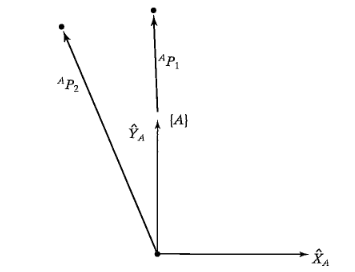
\includegraphics[width=0.5\columnwidth]{imgs/rotation_operator}
\end{figure}

\subsubsection{Transformation operators}
Let $^AP_1$ be a vector that is rotated and translated by the operator $T$. \\
The result of the operation is a new vector $^AP_2$ calculated as:
$$
	^AP_2 = T ⋅~^AP_1
$$
where
$$
	T = \left[\begin{array}{c|c}
	R_K(\theta) & Q \\ \hline 0~ 0~ 0 & 1
	\end{array}\right]
$$
and $R_K(\theta)$ is a rotational operator and $Q$ is a translational vector

%TODO proof

\subsection{Transformation arithmetic}
\subsubsection{Compound transformations}
Let $^A_BT$ and $^B_CT$ be homogeneous transforms. \\
Then $^A_CT$ is defined as: \\
$$
	^A_CT := ~^A_BT ⋅~ ^B_CT = \left[\begin{array}{c|c}
		^A_BR ⋅~^B_CR & ^A_BR ⋅~^BP_{CORG} + ~^AP_{BORG} \\
		\hline
		0 ~0 ~0 & 1
	\end{array}\right]
$$

\subsubsection{Inverting a transform}
Let $^A_BT$ be a transform. \\
Then $^B_AT$ is defined as: \\
$$
	^B_AT := ~^A_BT^{-1} = \left[\begin{array}{c|c}
	^A_BR^T & -^A_BR^T ⋅~^AP_{BORG} \\
	\hline
	0 ~0 ~0 & 1
	\end{array}\right]
$$

\subsection{More on representation of orientation}
\subsubsection{X-Y-Z fixed angles}
Let $^A_BR_{XYZ}(\gamma,\beta,\alpha)$ be a rotation matrix that describes a frame $\{B\}$ relative to a frame $\{A\}$ by a rotation about $\hat{X}_A$ by an angle $\gamma$, then about $\hat{Y}_A$ by an angle $\beta$ and finally about $\hat{Z}_A$ by an angle $\alpha$. \\
Then $^A_BR_{XYZ}(\gamma,\beta,\alpha)$ is defined as:
$$
	^A_BR_{XYZ}(\gamma,\beta,\alpha) = R_Z(\alpha) ⋅ R_Y(\beta) ⋅ R_X(\gamma) = \begin{bmatrix}
		\cos \alpha \cos \beta & \cos \alpha \sin \beta \sin \gamma - \sin \alpha \cos \gamma & \cos \alpha \sin \beta \cos \gamma + \sin \alpha \sin \gamma \\
		\sin \alpha \cos \beta & \sin \alpha \sin \beta \sin \gamma + \cos \alpha \cos \gamma & \sin \alpha \sin \beta \cos \gamma - \cos \alpha \sin \gamma \\
		- \sin \beta & \cos \beta \sin \gamma & \cos \beta \cos \gamma
	\end{bmatrix}
$$
\\

Let $^A_BR_{XYZ}(\gamma, \beta, \alpha) = \vect{r_{11} & r_{12} & r_{13} \\ r_{21} & r_{22} & r_{23} \\ r_{31} & r_{32} & r_{33}}$ be a rotation matrix (same conditions as above). \\
Then $\alpha$, $\beta$ and $\gamma$ are calculated as:
$$
	\beta = \atan (-r_{31}, \sqrt{r_{11}^2 + r_{21}^2})
$$
$$
	\alpha = \atan (\frac{r_{21}}{\cos \beta}, \frac{r_{11}}{\cos \beta})
$$
$$
	\gamma = \atan (\frac{r_{32}}{\cos \beta}, \frac{r_{33}}{\cos \beta})
$$

\subsubsection{Z-Y-X Euler angles}
Let $^A_BR_{Z'Y'X'}(\alpha, \beta, \gamma)$ be a rotation matrix that describes a frame $\{B\}$ relative to a frame $\{A\}$ by a rotation about $\hat{Z}_B$ by an angle $\alpha$, then about $\hat{Y}_B$ by an angle $\beta$ and finally about $\hat{X}_B$ by an angle $\gamma$. \\
Then $^A_BR_{Z'Y'X'}(\alpha, \beta, \gamma)$ is defined as:
$$
^A_BR_{Z'Y'X'}(\alpha, \beta, \gamma) = R_Z(\alpha) ⋅ R_Y(\beta) ⋅ R_X(\gamma) = \begin{bmatrix}
\cos \alpha \cos \beta & \cos \alpha \sin \beta \sin \gamma - \sin \alpha \cos \gamma & \cos \alpha \sin \beta \cos \gamma + \sin \alpha \sin \gamma \\
\sin \alpha \cos \beta & \sin \alpha \sin \beta \sin \gamma + \cos \alpha \cos \gamma & \sin \alpha \sin \beta \cos \gamma - \cos \alpha \sin \gamma \\
- \sin \beta & \cos \beta \sin \gamma & \cos \beta \cos \gamma
\end{bmatrix}
$$

\subsubsection{Z-Y-Z fixed angles}
Let $^A_BR_{Z'Y'Z'}(\alpha, \beta, \gamma)$ be a rotation matrix that describes a frame $\{B\}$ relative to a frame $\{A\}$ by a rotation about $\hat{Z}_B$ by an angle $\alpha$, then about $\hat{Y}_B$ by an angle $\beta$ and finally about $\hat{Z}_b$ by an angle $\gamma$. \\
Then $^A_BR_{Z'Y'Z'}(\alpha, \beta, \gamma)$ is defined as:
$$
^A_BR_{Z'Y'Z'}(\alpha, \beta, \gamma) = \begin{bmatrix}
\cos \alpha \cos \beta \cos \gamma - \sin \alpha \sin \gamma & - \cos \alpha \cos \beta \sin \gamma - \sin \alpha \cos \gamma & \cos \alpha \sin \beta \\
\sin \alpha \cos \beta \cos \gamma + \cos \alpha \sin \gamma & -\sin \alpha \cos \beta \sin \gamma + \cos \alpha \cos \gamma & \sin \alpha \sin \beta \\
- \sin \beta \cos \gamma & \sin \beta \sin \gamma & \cos \beta
\end{bmatrix}
$$
\\

Let $^A_BR_{Z'Y'Z'}(\alpha, \beta, \gamma) = \vect{r_{11} & r_{12} & r_{13} \\ r_{21} & r_{22} & r_{23} \\ r_{31} & r_{32} & r_{33}}$ be a rotation matrix (same conditions as above). \\
Then $\alpha$, $\beta$ and $\gamma$ are calculated as:
$$
\beta = \atan (\sqrt{r_{31}^2 + r_{32}^2}, r_{33})
$$
$$
\alpha = \atan (\frac{r_{23}}{\sin \beta}, \frac{r_{13}}{\sin \beta})
$$
$$
\gamma = \atan (\frac{r_{32}}{\sin \beta}, -\frac{r_{31}}{\sin \beta})
$$

\subsubsection{Equivalent angle-axis}
\paragraph{Same origin} ~\\
Let $\{A\}$ and $\{B\}$ be two frames with the same origin, where $\{B\}$ is rotated relative to $\{A\}$ about a vector $\hat{K} = \vect{k_x \\ k_y \\ k_z}$ by $\theta$ degrees . ($K$ goes through the origin) \\
Then the rotation matrix $^A_BR(\hat{K},\theta)$ is defined as: \\
$$
	^A_BR(\hat{K}, \theta) = R_K(\theta) = \begin{bmatrix}
		k_xk_x (1 - \cos \theta) + \cos \theta & k_xk_y(1 - \cos \theta) - k_z \sin \theta & k_xk_z(1 - \cos \theta) + k_y \sin \theta \\
		k_xk_y (1 - \cos \theta) + k_z \sin \theta & k_yk_y(1 - \cos \theta) + \cos \theta & k_yk_z(1 - \cos \theta) - k_x \sin \theta \\
		k_xk_z (1 - \cos \theta) - k_y \sin \theta & k_yk_z(1 - \cos \theta) + k_x \sin \theta & k_zk_z(1 - \cos \theta) + \cos \theta \\		
	\end{bmatrix}
$$

Let $^A_BR_K(\theta) = \vect{r_{11} & r_{12} & r_{13} \\ r_{21} & r_{22} & r_{23} \\ r_{31} & r_{32} & r_{33}}$ be a rotation matrix (same conditions as above). \\
Then $\theta$ and $\hat{K}$ are calculated as:
$$
	\theta = \arccos \left(\frac{r_{11} + r_{22} + r_{33} - 1}{2}\right)
$$
$$	
	\hat{K} = \frac {1}{2 \sin \theta} \vect{r_{32} - r_{23} \\ r_{13} - r_{31} \\ r_{21} - r_{12}} \text{, if } \theta ≠ 0° \text{ and } \theta ≠ 180°
$$

\paragraph{Different origins} ~\\
Let $\{A\}$ and $\{B\}$ be two frames, where $\{B\}$ is rotated relative to $\{A\}$ about a vector $\hat{K} = \vect{k_x \\ k_y \\ k_z}$ by $\theta$ degrees. $\hat{K}$ passes through the point $^AP$ \\
Then the translation matrix $^A_BR(\hat{K},\theta)$ is defined as: \\
$$
^A_BR(\hat{K}, \theta) = ^A_{A'}T ⋅~^{A'}_{B'}T ⋅~^{B'}_BT
$$
where $^A_{A'}T = \left[\begin{array}{c|c}
	I_3 & ^AP \\
	\hline
	0 ~0 ~0 & 1
\end{array}\right]$, 
$^B_{B'}T = \left[\begin{array}{c|c}
I_3 & -^AP \\
\hline
0 ~0 ~0 & 1
\end{array}\right]$ \\
and $\{A'\}$ and $\{B'\}$ are frames with the same origin as $\hat{K}$ and the same orientation as $\{A\}$ and $\{B\}$.

\subsubsection{Euler parameters}
Let $\hat{K} = \vect{k_x \\ k_y \\ k_z}$ be a equivalent axis and $\theta$ be the equivalent angle.
Then the Euler parameters are given by: \\
$$
	\epsilon_1 = k_x \sin \frac \theta 2
$$
$$
	\epsilon_2 = k_y \sin \frac \theta 2
$$
$$
	\epsilon_3 = k_z \sin \frac \theta 2
$$
$$
	\epsilon_4 = \cos \frac \theta 2
$$
It follows: \\
$$
	\epsilon_1^2 + \epsilon_2^2 + \epsilon_3^2 + \epsilon_4^2 = 1
$$
The rotation matrix $R_\epsilon$ is defined as:
$$
	R_\epsilon = \begin{bmatrix}
		1 - 2\epsilon_2^2 - 2\epsilon_3^2 & 2(\epsilon_1\epsilon_2 - \epsilon_3\epsilon_4) & 2(\epsilon_1\epsilon_3 + \epsilon_2\epsilon_4) \\
		2(\epsilon_1\epsilon_2 + \epsilon_3\epsilon_4) & 1 - 2\epsilon_1^2 - 2\epsilon_3^2 & 2(\epsilon_2\epsilon_3 - \epsilon_1\epsilon_4) \\
		2(\epsilon_1\epsilon_3 - \epsilon_2\epsilon_4) & 2(\epsilon_2\epsilon_3 + \epsilon_1\epsilon_4) & 1 - 2\epsilon_1^2 - 2\epsilon_2^2
	\end{bmatrix}
$$
Given a rotation matrix, the equivalent Euler parameters are:
$$
	\epsilon_1 = \frac{r_{32} - r_{23}}{4\epsilon_4}
$$
$$
	\epsilon_2 = \frac{r_{13} - r_{31}}{4\epsilon_4}
$$
$$
	\epsilon_3 = \frac{r_{21} - r_{12}}{4\epsilon_4}
$$
$$
	\epsilon_4 = \frac 1 2 \sqrt{1 + r_{11} + r_{22} + r_{33}}
$$

\subsection{Vectors}
\subsubsection{Equality}
Two vectors are equal if they have the same dimension, magnitude and direction

\subsubsection{Equivalence}
Two vectors are equivalent in a certain capacity if each produces the very same effect in this capacity

\subsubsection{line vector}
A line vector refers to a vector that is dependent on its line of action, along with direction and magnitude, for causing effects

\subsubsection{Free vector}
A free vector is a vector that may be positioned anywhere in space without loss or change of meaning, provided that magnitude and direction are preserved

\section{Forward Kinematics}
\begin{itemize}
	\item Science of motion that treats the subject without regard to the forces that cause it.
	\item compute the position and orientation of the manipulator's end-effector relative to the base of the manipulator as a function of the joint variables
\end{itemize}

\subsection{Link description}
\subsubsection{Joints}
\begin{figure}[H]
	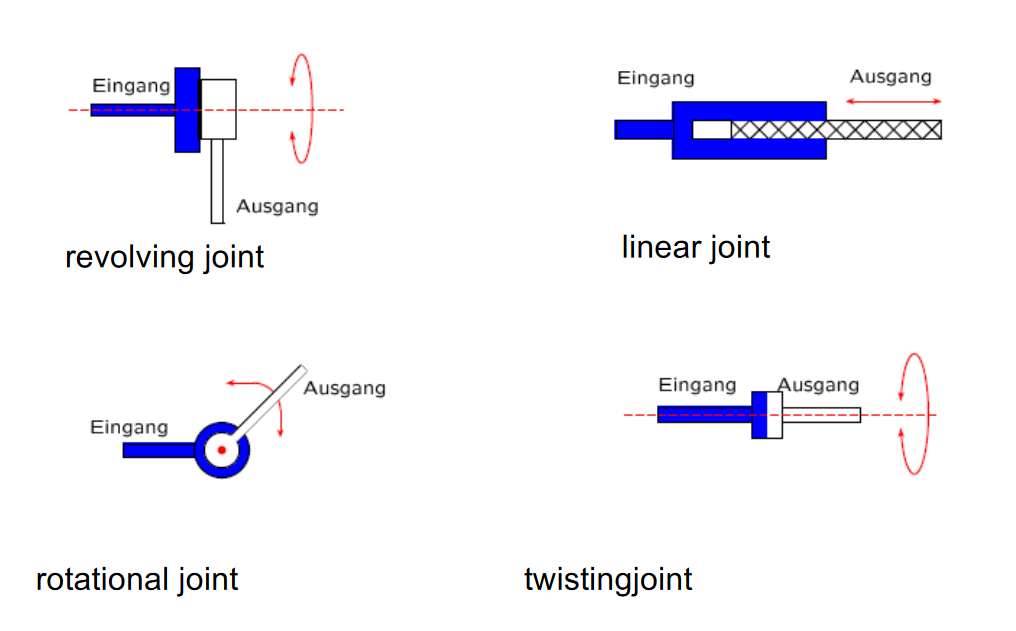
\includegraphics[width=1\columnwidth]{imgs/joints}
\end{figure}

\subsubsection{Lower pair joints}
\begin{figure}[H]
	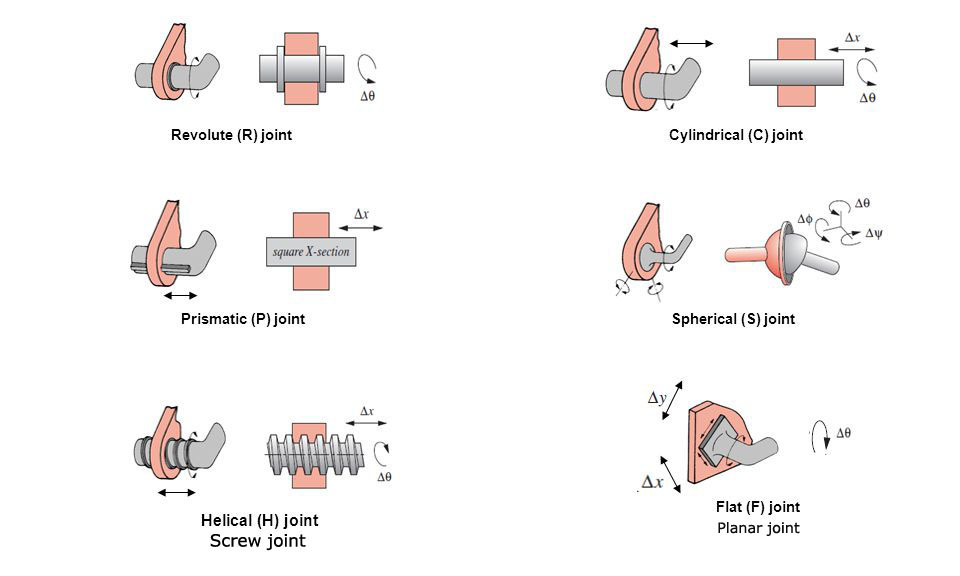
\includegraphics[width=1\columnwidth]{imgs/lower_pair_joints1.jpg}
\end{figure}

\subsubsection{Link}
\begin{itemize}
	\item body connected in a chain by joints
	\item a link is considered only as a rigid body that defines the relationship between two neighboring joint axes of a manipulator
\end{itemize}

\subsubsection{Numbering of links}
\begin{itemize}
	\item Starting from the base: link 0, link 2, $\dots$, link $n$
	\item First moving body is link 1
\end{itemize}

\subsubsection{Link length}
Let link $i-1$ be a link with two axes Axis $i-1$ and Axis $i$. \\
The measure of distance of a line that is mutually orthogonal to both axes is called link length $a_{i-1}$

\subsubsection{Link twist}
Let link $i-1$ be a link with two axes Axis $i-1$ and Axis $i$ and the link length $a_{i-1}$. \\
The angle that is measured from axis $i-1$ to axis $i$ in the right-hand sense about $a_{i-1}$ is called link twist $\alpha_{i-1}$

\subsection{Link-connection description}
\subsubsection{Link offset}
Let link $i-1$ and link $i$ be two links with the common joint axis Axis $i$. \\
The distance along this common axis from the link $i-1$ to the link $i$ is called link offset $d_i$ \\

\subsubsection{Joint angle}
Let link $i-1$ and link $i$ be two links with the common joint axis Axis $i$. \\
The amount of rotation about this common axis between the link $i-1$ and link $i$ is called joint angle $\theta_i$ (right-hand sense)

\begin{figure}[H]
	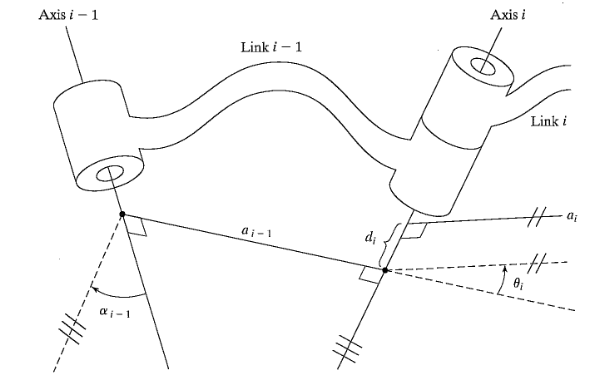
\includegraphics[width=0.5\columnwidth]{imgs/link_connection.png}
\end{figure}

\subsubsection{First and last links in the chain}
Let link $0$ be the first link and link $n$ be the last link. It follows: \\
$$
	a_0 = a_n = 0
$$
$$
	\alpha_0 = \alpha_n = 0
$$

\subsubsection{Revolute/Rotational Joints}
Let joint $i$ be a revolute joint. It follows: \\
$d_i = 0$ and $\theta_i$ is called the joint variable

\subsubsection{Prismatic/Linear Joints}
Let joint $i$ be a prismatic joint. It follows: \\
$\theta_i = 0$ and $d_i$ is called the joint variable

\subsubsection{Denavit-Hartenberg notation}
\begin{itemize}
	\item Description of any robot kinematically by giving the values of four quantities for each link. Two describing the link itself ($a_0, \dots, a_{n-1}$ and $\alpha_0, \dots, \alpha_{n-1}$) and two describing the link's connection to a neighboring link ($d_0, \dots, d_n$ and $\theta_0, \dots, \theta_i$): \\
	
	$\begin{array}{|c|c|c|c|c|}
	\hline
		i & \alpha_{i-1} & a_{i-1} & d_i & \theta_i \\
		\hline
		\hline
		1 & \alpha_0 & a_0 & d_1 & \theta_1 \\
		\hline
		2 & \alpha_1 & a_1 & d_2 & \theta_2 \\
		\hline
		\multicolumn{5}{|c|}{\vdots} \\
		\hline
		n & \alpha_{n-1} & a_{n-1} & d_n & \theta_n \\
		\hline
	\end{array}$
\end{itemize}

\subsection{Convention for affixing frames to links}
\subsubsection{Attach a frame to a link}
Let link $i$ be a link with two axes Axis $i$ and Axis ${i+1}$ and the link length $a_i$. \\
The frame $\{i\}$ will be located on the link as follows:
\begin{description}
	\item The $\hat{Z}$-axis of frame $\{i\}$ is called $\hat{Z}_i$ and is coincident with the Axis $i$
	\item The origin of frame $\{i\}$ is located where the $a_i$ orthogonal intersects the Axis $i$
	\item The $\hat{X}$-axis of frame $\{i\}$ is called $\hat{X}_i$ and points along $a_i$ in the direction from Axis $i$ to Axis $i+1$
	\item The link twist $\alpha_i$ is measured in the right-hand sense about $\hat{X}_i$
	\item The $\hat{Y}$-axis of frame $\{i\}$ is called $\hat{Y}_i$ and is formed by the right-hand rule
\end{description}

\begin{figure}[H]
	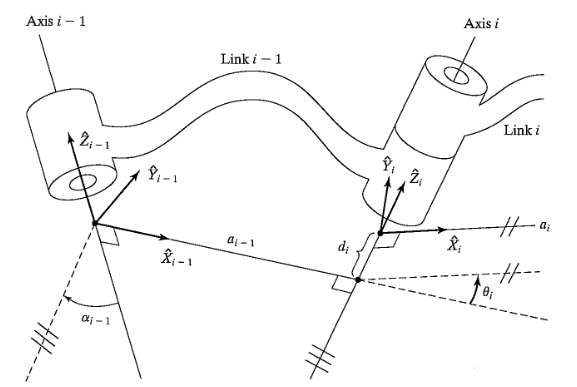
\includegraphics[width=0.5\columnwidth]{imgs/link_frame.png}
\end{figure}

\subsubsection{Base frame}
The frame attached to the base of the robot, or link 0, is called frame $\{0\}$ and doesn't move.

\subsubsection{Link parameters in terms of the link frames}
$$
	a_i = \text{the distance from } \hat{Z}_i \text{ to } \hat{Z}_{i+1} \text{ measured along } \hat{X}_i
$$
$$
	\alpha_i = \text{the angle from } \hat{Z}_i \text{ to } \hat{Z}_{i+1} \text{ measured about } \hat{X}_i
$$
$$
	d_i = \text{the distance from } \hat{X}_{i-1} \text{ to } \hat{X}_i \text{ measured along } \hat{Z}_i
$$
$$
	\theta_i = \text{the angle from } \hat{X}_{i-1} \text{ to } \hat{X}_i \text{ measured about } \hat{Z}_i
$$

\subsubsection{Link-Frame Attachment Procedure}
The following is a summary of the procedure to follow when faced with a new mechanism, in order to properly attach the link frames:
\begin{enumerate}
	\item Identify the joint axes and imagine (or draw) infinite lines along them. steps 2 through 5 below, consider two of these neighboring lines (at axes $i$ and $i + 1$).
	\item Identify the common perpendicular between them, or point of intersection. At the point of intersection, or at the point where the common perpendicular meets the $i$-th axis, assign the link-frame origin. 
	\item Assign the $\hat{Z}_1$ axis pointing along the $i$-th joint axis. 
	\item Assign the $\hat{X}_i$ axis pointing along the common perpendicular, or, if the axes intersect, assign $\hat{X}_i$ to be normal to the plane containing the two axes. 
	\item Assign the $\hat{Y}_i$ axis to complete a right-hand coordinate system. 
	\item Assign $\{0\}$ to match $\{1\}$ when the first joint variable is zero. For $\{N\}$, choose an origin location and $\hat{X}_N$ direction freely, but generally so as to cause as many linkage parameters as possible to become zero.
\end{enumerate}

\subsection{Forward Kinematics}
\subsubsection{Link transformations}
Let $^{i-1}_iT$ be the transform that defines frame $\{i\}$ relative to frame $\{i-1\}$. \\
Let $\{P\}$, $\{Q\}$ and $\{R\}$ be frames where \\
\tab frame $\{R\}$ differs from frame $\{i-1\}$ by a rotation of $\alpha_{i-1}$, \\
\tab frame $\{Q\}$ differs from frame $\{R\}$ by a translation $a_{i-1}$, \\
\tab frame $\{P\}$ differs from frame $\{Q\}$ by a rotation $\theta_i$ and \\
\tab frame $\{i\}$ differs from frame $\{P\}$ by a translation $d_i$. \\
$^{i-1}_iT$ is calculated as: \\
$$
\begin{multlined}
	^{i-1}_iT = ~^{i-1}_RT ⋅ ~^R_QT ⋅ ~^Q_PT ⋅ ~^P_iT = R_X(\alpha_{i-1}) ⋅ D_X(a_{i-1}) ⋅ R_Z(\theta_i) ⋅ D_Z(d_i) \\ \\
	= \begin{bmatrix}
		\cos \theta_i & -\sin \theta_i & 0 & a_{i-1} \\
		\sin \theta_i \cos \alpha_{i-1} & \cos \theta_i \cos \alpha_{i-1} & -\sin \alpha_{i-1} & -\sin \alpha_{i-1} d_i \\
		\sin \theta_i \sin \alpha_{i-1} & \cos \theta_i \sin \alpha_{i-1} & \cos \alpha_{i-1} & \cos \alpha_{i-1} d_i \\
		0 & 0 & 0 & 1		
	\end{bmatrix}
\end{multlined}
$$

\subsubsection{Concatenating link transformations}
Let $^{i-1}_iT$ be the transform that defines frame $\{i\}$ relative to frame $\{i-1\}$ and let frame $\{0\}$ be the first frame and $\{N\}$ be the last frame. \\
$^0_NT$ is calculated as:
$$
	^0_NT = ~^0_1T ⋅ ~^1_2T ⋅ \dots ⋅ ~^{N-1}_NT
$$

\subsection{Frames With Standard Names}
\subsubsection{Base Frame \{B\}}
\begin{itemize}
	\item is located at the base of the manipulator
	\item Another name for frame $\{0\}$
	\item Affected to a non-moving part of the robot (sometimes called link 0)
\end{itemize}

\subsubsection{Station Frame \{S\}}
\begin{itemize}
	\item is located in a task-relevant location (e.g at the corner of a table)
	\item if the user of this robot is concerned, $\{S\}$ is the universe frame
	\item Also called: task/world/universe frame
	\item specified relative to the base frame: $^B_ST$
\end{itemize}

\subsubsection{Wrist Frame \{W\}}
\begin{itemize}
	\item is affixed to the last link of the manipulator
	\item Another name for frame $\{N\}$
	\item Often $\{W\}$ has its origin fixed at a point called the wrist of the manipulator
	\item specified relative to the base frame: $^B_WT = ~^0_NT$ 
\end{itemize}
\subsubsection{Tool Frame \{T\}}
\begin{itemize}
	\item is affixed to the end of any tool the robot happens to be holding
	\item When the hand is empty $\{T\}$ is usually located with its origin between the fingertips of the robot
	\item specified relative to the wrist frame: $^W_TT$
\end{itemize}
\subsubsection{Goal Frame \{G\}}
\begin{itemize}
	\item is a description of the location to which the robot is to move the tool
	\item specified relative to the station frame: $^S_GT$
\end{itemize}

\begin{figure}[H]
	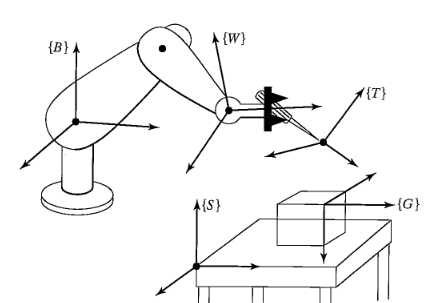
\includegraphics[width=0.5\columnwidth]{imgs/standard_frames.png}
\end{figure}

\subsection{WHERE is the tool}
Let $\{B\}$ be the base frame, $\{S\}$ be the station frame, $\{W\}$ be the wrist frame and $\{T\}$ be the tool frame. \\
The WHERE function in some robot system computes where the tool is relative to the station. That is computed as: \\
$$
	^S_TT = ~^B_ST^{-1} ⋅ ~^B_WT ⋅ ~^W_TT
$$

\section{Inverse Kinematics}
\subsection{Solvability}
\begin{itemize}
	\item All Systems with revolute and prismatic joints having a total of six degrees of freedom in a single series chain are solvable
\end{itemize}
\subsubsection{One Solution}
\begin{itemize}
	\item If the desired position and orientation of the wrist frame is in the workspace, then at least one solution exists.
\end{itemize}

\subsubsection{Multiple Solutions}
\begin{itemize}
	\item The chosen solution depends on several criteria e.g:
	\begin{itemize}
		\item Nearest solution
		\item Obstacles
		\item Link lengths and weights
	\end{itemize}
	\item Number of solutions of a manipulator with six rotational joints: \\
	\begin{tabular}{|c|c|}
		\hline
		$a_i$ & Number of solutions \\
		\hline
		$a_1 = a_3 = a_5 = 0$ & $≤4$ \\
		$a_3 = a_5 = 0$ & $≤8$ \\
		$a_3 = 0$ & $≤16$ \\
		all $a_i ≠ 0$ & $≤16$ \\	
		\hline
	\end{tabular}
	\end{itemize}

\subsubsection{Methods of Solution}
\begin{itemize}
	\item \textbf{numerical solutions:} generally much slower than closed-form solution
	\item \textbf{closed-form solutions:} 
	\begin{itemize}
		\item based on analytic expressions or on the solution of a polynomial of degree 4 or less
		\item Distinction between algebraic and geometric solution
	\end{itemize}
\end{itemize}

\subsection{The Notion of Manipulator Subspace when $n < 6$}
Let $^B_WT$ be the transformation matrix of the wrist frame relative to the base frame of a $n$-degree-of-freedom manipulator, where $n < 6$. The reachable workspace can be thought of as a portion of an $n$-degree-of-freedom subspace given by: \\
$$
	^B_WT
$$

\subsubsection{Specifying a general Goal for a manipulator when $n < 6$}
Let a general goal frame $^S_GT$ be given
\begin{enumerate}
	\item Compute a modified goal frame $^S_{G'}T$, such that $^S_{G'}$ lies in the manipulator's subspace and is as near to $^S_GT$ as possible
	\item Compute the inverse kinematics to find joint angles using $^S_{G'}$ as the desired goal
\end{enumerate}

\subsection{Algebraic solution}
Let $^B_WT$ be the Transformation matrix of a 3R planar manipulator with \\
$^B_WT = ^0_3T = \begin{bmatrix}
	c_{123} & -s_{123} & 0 & l_1c_1 + l_2c_{12} \\
	s_{123} & c_{123} & 0 & l_1s_1 + l_2s_{12} \\
	0 & 0 & 1 & 0 \\
	0 & 0 & 0 & 1
\end{bmatrix}$ \\
It follows:
$$
	\theta_2 = \atan(s_2,c_2)
$$
$$
	\theta_1 = \atan(y,x) - \atan(k_2,k_1)
$$
$$
	\theta_1 + \theta_2 + \theta_3 = \atan(s_{123}, c_{123})
$$, where
$$
	x = k_1c_1 - k_2s_1
$$
$$
	y = k_1s_1 + k_2c_1
$$
$$
	k_1 = l_1 + l_2c_2
$$
$$
	k_2 = l_2s_2
$$

\subsection{Geometric solution}
Let $^B_WT$ be the Transformation matrix of a 3R planar manipulator with \\
$^B_WT = ^0_3T = \begin{bmatrix}
c_\phi & -s_\phi & 0 & x \\
s_\phi & c_\phi & 0 & y \\
0 & 0 & 1 & 0 \\
0 & 0 & 0 & 1
\end{bmatrix}$ \\
It follows:
$$
	\cos \theta_2 = \frac{x^2 + y^2 - l_1^2 - l_2^2}{2 l_1 l_2}
$$
$$
	\theta_2' = -\theta_2
$$
$$
	\theta_1 = \atan(y,x) \pm \psi
$$
$$
	\theta_1 + \theta_2 + \theta_3 = \atan(s_\phi, c_\phi)
$$
,where
$$
	\cos \psi = \frac{x^2 + y^2 + l_1^2 - l_2^2}{2l_1 \sqrt{x^2 + y^2}}
$$

\subsection{Algebraic Solution by Reduction to Polynomial}
\label{inverse-substitution}
Make the following substitution:
$$
	u = \tan \frac \theta 2
$$
$$
	\cos \theta = \frac{1 - u^2}{1 + u^2}
$$
$$
	\sin \theta = \frac{2u}{1 + u^2}
$$
This substitution convert transcendental equations into polynomial equations in $u$ \\

Let the following transcendental  equation be given: \\
$a ⋅ \cos \theta + b ⋅ \sin \theta = c$ \\
$\theta$ is calculated as:
$$
	\theta = \atan(b,a) \pm \atan(\sqrt{a^2 + b^2 - c^2},c)
$$

\subsection{Pieper's solution when three axes intersect}
Let a manipulator be given with the following properties: \\
\begin{itemize}
	\item 6 degree of freedom
	\item all six joints are revolute
	\item the last three axes intersect
\end{itemize}
Let the origins of the link frames $\{4\}, \{5\}$ and $\{6\}$ be: \\
$^0P_{4ORG} = \vect{x \\ y \\ z}$ \\
Let further definitions be given as: \\
$f_1 = a_3c_3 + d_4s\alpha_3s_3 + a_2$ \\
$f_2 = a_3c\alpha_2s_3 - d_4s\alpha_3c\alpha_2c_3 - d_4s\alpha_2c\alpha_3 - d_3s\alpha_2$ \\
$f_3 = a_3s\alpha_2s_3 - d_4s\alpha_3s\alpha_2c_3 + d_4c\alpha_2c\alpha_3 + d_3c\alpha_2$ \\
$k_1 = f_1$ \\
$k_2 = -f_2$ \\
$k_3 = f_1^2 + f_2^2 + f_3^2 + a_1^2 + d_2^2 + 2d_2f_3$ \\
$k_4 = f_3c\alpha_1 + d_2c\alpha_1$ \\
and $r:= x^2 + y^2 + z^2$ \\
It follows: \\
$$
	r = (k_1c_2 + k_2s_2)2a_1 + k_3
$$
$$
	z = (k_1s_2 - k_2c_2)s\alpha_1 + k_4
$$

$\theta_3$ can be computed as follows:
\begin{itemize}
	\item If $a_1 = 0 \implies r = k_3$. Use substitution of section \ref{inverse-substitution}
	\item If $s\alpha_1 = 0 \implies z = k_4$. Use substitution of section \ref{inverse-substitution}
	\item Otherwise: $\frac{(r - k_3)^2}{4a_1^2} + \frac{(z - k_4)^2}{s^2\alpha_1} = k_1^2 + k_2^2$
\end{itemize}

$\theta_2$ can be computed using: \\
$$
r = (k_1c_2 + k_2s_2)2a_1 + k_3
$$
$$
z = (k_1s_2 - k_2c_2)s\alpha_1 + k_4
$$

$\theta_1$ can be computed using: \\
$$
	^0P_{4ORG} = \vect{c_1g_1 - s_1g_2 \\ s_1g_1 + c_1g_2 \\ g_3}
$$, where \\
$g_1 = c_2f_1 - s_2f_2 + a_1$ \\
$g_2 = s_2c\alpha_1f_1 + c_2c\alpha_1f_2 - s\alpha_1f_3 - d_2s\alpha_1$ \\
$g_3 = s_2s\alpha_1f_1 + c_2s\alpha_1f_2 + c\alpha_1f_3 + d_2c\alpha_1$ \\
and 
$$
	^4_6R|_{\theta_4 = 0} = ~^0_4R^{-1}|_{\theta_4 = 0} ⋅ ~^0_6R
$$

\subsection{Solve-ing a manipulator}
The SOLVE function implements Cartesian transformations and calls the inverse kinematic function. It calculates the location of $\{W\}$ relative to $\{B\}$: \\
$$
	^B_WT = ~^B_ST ⋅ ~^S_TT ⋅ ~^W_TT^{-1}
$$
Then, the inverse kinematics take $^B_WT$ as an input and calculate $\theta_1$ through $\theta_n$

\section{Jacobians: velocities and static forces}
\subsection{Notation for time-varying Position and Orientation}
\subsubsection{Differentiation of position vectors}
Let $^BQ$ be a position vector relative to frame $\{B\}$. \\
The velocity of $Q$ relative to frame $\{B\}$ is computed as the derivative of $^BQ$ w.r.t. time and defined as:
$$
	^BV_Q = \frac{d}{dt} ~^BQ = \lim_{\Delta t → 0} \frac{^BQ(t + \Delta t) - ~^BQ(t)}{\Delta t}
$$

Let $^BQ$ be a position vector relative to $\{B\}$ \\
The velocity vector of $^BQ$ expressed in terms of frame $\{A\}$ is calculated as:
$$
	^A(^BV_Q) = ~^A_BR ⋅ ~^BV_Q = \frac{^Ad}{dt}⋅ ~^BQ
$$, where the velocity (done by the derivation) is relative to frame $\{B\}$ but the velocity vector itself is expressed in terms of frame $\{A\}$ and
$$
	^B(^BV_Q) = ~^BV_Q
$$

Let $^UCORG$ be the origin of frame $\{C\}$ relative to frame $\{U\}$ \\
The velocity of $^UCORG$ relative to the universe frame $\{U\}$ is defined as:
$$
	v_C = ~^UV_{CORG}
$$
and the velocity vector of $^UCORG$ expressed int terms of frame $\{A\}$ (though differentiation done relative to $\{U\}$) is defined as:
$$
	^Av_C = ~^A_UR ⋅ v_C
$$

\subsubsection{Angular velocity vector}
Let $\{A\}$ and $\{B\}$ be two frames. \\
The angular velocity of a rotation of frame $\{B\}$ relative to $\{A\}$ is defined as:
$$
^A\Omega_B
$$
, where the direction of $^A\Omega_B$ indicates the axis of rotation \\
and the magnitude of $^A\Omega_B$ indicates the speed of rotation \\

Let $^A\Omega_B$ be an angular velocity vector \\
$^A\Omega_B$ expressed in terms of a frame $\{C\}$ is defined as:
$$
^C(^A\Omega_B)
$$, where the rotation of frame $\{B\}$ is relative to frame $\{A\}$ but the angular velocity vector itself is expressed in terms of frame $\{C\}$ \\

Let $\{C\}$ be a frame and $\{U\}$ be the universe frame \\
The angular velocity of a rotation of frame $\{C\}$ relative to $\{U\}$ is defined as:
$$
\omega_C = ~^U\Omega_{C}
$$
and the angular velocity vector of $\{C\}$ relative to $\{U\}$ expressed in terms of frame $\{A\}$ is defined as:
$$
^A\omega_C
$$

\subsection{Linear and Rotational Velocity of rigid bodies}
\subsubsection{Linear Velocity}
Let $\{A\}$ and $\{B\}$ be two frames \\
and $^BQ$ a position vector relative to $\{B\}$ which may change with time \\
Let the location of $\{B\}$ relative to $\{A\}$ be described by a position vector $^AP_{BORG}$ which may change with time \\
and a rotation matrix $^A_BR$ which is not changing with time \\
The velocity of $Q$ relative to $\{A\}$ is computed as: \\
$$
	^AV_Q = ~^AV_{BORG} + ~^A_BR⋅ ~^BV_Q
$$
, where $^AV_{BORG}$ is the linear velocity of frame $\{B\}$ relative to $\{A\}$

\begin{figure}[H]
	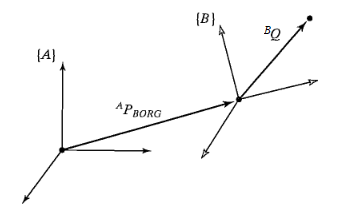
\includegraphics[width=0.5\columnwidth]{imgs/velocity_trans.png}
\end{figure}

\subsubsection{Rotational velocity}
Let $\{A\}$ and $\{B\}$ be two frames with the same origins and with zero linear relative velocity \\
Let $^BQ$ be a position vector relative to $\{B\}$ which may change with time \\
Let $^A\Omega_B$ be a vector describing the rotational velocity of $\{B\}$ relative to $\{A\}$ \\
Let $^A_BR$ a rotation matrix describing $\{B\}$ relative to $\{A\}$ \\
The velocity of $Q$ relative to $\{A\}$ is computed as: \\
$$
	^AV_Q = ~^A_BR ⋅~^BV_Q + ~^A\Omega_B \times ~^A_BR ⋅ ~^BQ
$$

\begin{figure}[H]
	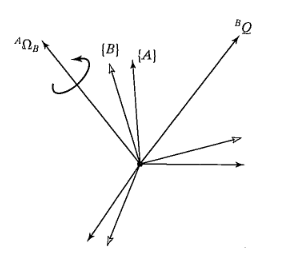
\includegraphics[width=0.5\columnwidth]{imgs/velocity_rot.png}
\end{figure}

\subsubsection{Simultaneous linear and rotational velocity}
Let $\{A\}$ and $\{B\}$ be two frames \\
Let $^BQ$ be a position vector relative to $\{B\}$ which may change with time \\
Let the location of $\{B\}$ relative to $\{A\}$ be described by a position vector $^AP_{BORG}$ which may change with time \\
Let $^A\Omega_B$ be a vector describing the rotational velocity of $\{B\}$ relative to $\{A\}$ \\
Let $^A_BR$ a rotation matrix describing $\{B\}$ relative to $\{A\}$ \\
The velocity of $Q$ relative to $\{A\}$ is computed as: \\
$$
^AV_Q = ~^AV_{BORG} + ~^A_BR ⋅~^BV_Q + ~^A\Omega_B \times ~^A_BR ⋅ ~^BQ
$$

\subsection{More on Angular Velocity}
\subsubsection{Other representations of angular velocity}
\paragraph{Z-Y-Z Euler angles} ~\\
$$
	\dot \Theta_{Z'Y'Z'} = \vect{\dot \alpha \\ \dot \beta \\ \dot \gamma}
$$

\subsection{Velocity "Propagation" from link to link}
\subsubsection{Rotational joints}
Let joint $i+1$ be rotational: \\

Let $^{i+1}_iR$ a rotation matrix describing $\{i\}$ relative to $\{i+1\}$ \\
Let $^i\omega_i$ be the angular velocity vector of link $\{i\}$ relative to $\{B\}$ expressed in terms of frame $\{i\}$ \\
The angular velocity of link $i + 1$ with respect to frame $\{i + 1\}$ is calculated as:
$$
	^{i+1}\omega_{i+1} = ~^{i+1}_iR ⋅ ~^i\omega_i + \dot \theta_{i+1} ⋅ ~^{i+1}\hat{Z}_{i+1}
$$
, where $\dot \theta_{i+1} ⋅ ^{i+1}\hat{Z}_{i+1} = ~^{i+1}\vect{0 \\ 0 \\ \dot{\theta}_{i+1}}$ \\
\\

Let $^{i+1}_iR$ a rotation matrix describing $\{i\}$ relative to $\{i+1\}$ \\
Let $^iv_i$ be the linear velocity of the origin of link $\{i\}$ relative to $\{B\}$ expressed in terms of frame $\{i\}$ \\
Let $^i\omega_i$ be the angular velocity vector of link $\{i\}$ relative to $\{B\}$ expressed in terms of frame $\{i\}$ \\
Let $^iP_{i+1}$ be the origin of $\{i+1\}$ relative to $\{i\}$
The linear velocity of link $i + 1$ with respect to frame $\{i + 1\}$ is calculated as:
$$
	^{i+1}v_{i+1} = ~^{i+1}_iR(^iv_i + ~^i\omega_i \times ~^iP_{i+1})
$$

\subsubsection{Prismatic joints}
Let joint $i+1$ be prismatic: \\

Let $^{i+1}_iR$ a rotation matrix describing $\{i\}$ relative to $\{i+1\}$ \\
Let $^i\omega_i$ be the angular velocity vector of link $\{i\}$ relative to $\{B\}$ expressed in terms of frame $\{i\}$ \\
The angular velocity of link $i + 1$ with respect to frame $\{i + 1\}$ is calculated as:
$$
	^{i+1}\omega_{i+1} = ~^{i+1}_iR ⋅ ~^i\omega_i
$$

Let $^{i+1}_iR$ a rotation matrix describing $\{i\}$ relative to $\{i+1\}$ \\
Let $^iv_i$ be the linear velocity of the origin of link $\{i\}$ relative to $\{B\}$ expressed in terms of frame $\{i\}$ \\
Let $^i\omega_i$ be the angular velocity vector of link $\{i\}$ relative to $\{B\}$ expressed in terms of frame $\{i\}$ \\
Let $^iP_{i+1}$ be the origin of $\{i+1\}$ relative to $\{i\}$
The linear velocity of link $i + 1$ with respect to frame $\{i + 1\}$ is calculated as:
$$
	^{i+1}v_{i+1} = ~^{i+1}_iR(^iv_i + ~^i\omega_i \times ~^iP_{i+1}) + \dot{d}_{i+1} ⋅ ~^{i+1}\hat{Z}_{i+1}
$$

\begin{figure}[H]
	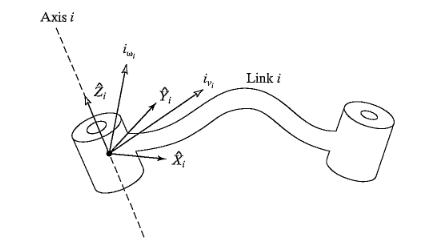
\includegraphics[width=0.5\columnwidth]{imgs/velocity_link.png}
\end{figure}

\subsection{Jacobians}
\subsubsection{Jacobian-Matrix}
$$
	\mathcal{J}(\Theta) = \begin{bmatrix}
		\frac{\partial f_1}{\partial \theta_1} & \dots & \frac{\partial f_1}{\partial \theta_n} \\
		\vdots & \ddots & \vdots \\
		\frac{\partial f_m}{\partial \theta_1} & \dots & \frac{\partial f_m}{\partial \theta_n} \\
	\end{bmatrix}
$$
, with $\Theta = \vect{\theta_1 \\ \vdots \\ \theta_n}$

\subsubsection{Relate Joint Velocities to Cartesian Velocities}
$$
	^i\nu = \vect{^iv \\ ^i\omega} = ~^i\mathcal{J}(\Theta) ⋅ \dot{\Theta}
$$
, where $^i\nu$ is a vector of Cartesian velocities (here: of the end-effector frame relative to $\{B\}$): A linear velocity vector expressed in terms of $\{i\}$ and a rotational velocity vector expressed in $\{i\}$. and \\
$\Theta = \vect{\theta_1 \\ \vdots \\ \theta_n}$ \\

Dimension of the Jacobian Matrix:
\begin{itemize}
	\item Number of rows $\hat{=}$ Number of degrees of freedom in the Cartesian space ($\times 2$ for velocity and angular velocity)
	\item Number of columns $\hat{=}$ Number of joints of the manipulator
\end{itemize}

\subsubsection{Changing a Jacobian's frame of reference}
Let $^B\mathcal{J}(\Theta)$ be a Jacobian written in frame $\{B\}$ (with $^B\nu  = ~^B\mathcal{J}(\Theta)\dot \Theta$)\\
The Jacobian written in $\{A\}$ is computed as: \\
$$
	^A\mathcal{J}(\Theta) = \left[\begin{array}{c|c}
		^A_BR & 0 \\
		\hline
		0 & ^A_BR
	\end{array}\right] ⋅ ~^B\mathcal{J}(\Theta)
$$

\paragraph{Example} ~\\
Let $^nv_n = \begin{bmatrix}
	\alpha_{11} \dot{\theta}_1 + & \dots & + \alpha_{1n} \dot{\theta}_n \\
	\alpha_{21} \dot{\theta}_1 + & \dots & + \alpha_{2n} \dot{\theta}_n \\
	\alpha_{31} \dot{\theta}_1 + & \dots & + \alpha_{3n} \dot{\theta}_n \\	
\end{bmatrix}$ be a velocity vector of frame $\{n\}$ relative to $\{B\}$ expressed in $\{n\}$ and \\
let $^n\omega_n = \begin{bmatrix}
\beta_{11} \dot{\theta}_1 + & \dots & + \beta_{1n} \dot{\theta}_n \\
\beta_{21} \dot{\theta}_1 + & \dots & + \beta_{2n} \dot{\theta}_n \\
\beta_{31} \dot{\theta}_1 + & \dots & + \beta_{3n} \dot{\theta}_n \\	
\end{bmatrix}$ be an angular velocity vector of frame $\{n\}$ relative to $\{B\}$ expressed in $\{n\}$ and \\
let $\dot{\Theta} = \vect{\dot \theta_1 \\ \vdots \\ \dot \theta_n}$ \\
It follows: \\
$$
	^n\nu = \vect{^nv \\ ^n\omega} = ~^n\mathcal{J}(\Theta) ⋅ \dot{\Theta} = \begin{bmatrix}
		\alpha_{11} & \dots & \alpha_{1n} \\
		\alpha_{21} & \dots & \alpha_{2n} \\
		\alpha_{31} & \dots & \alpha_{3n} \\
		\beta_{11} & \dots & \beta_{1n} \\
		\beta_{21} & \dots & \beta_{2n} \\
		\beta_{31} & \dots & \beta_{3n} \\
	\end{bmatrix} ⋅ \vect{\dot{\theta}_1 \\ \vdots \\ \dot{\theta}_n}
$$

\subsection{Singularity}
\subsubsection{Categories}
\begin{itemize}
	\item \textbf{Workspace-boundary singularities} occur when the manipulator is fully stretched out or folded back on itself in such a way that the end-effector is at or very near the boundary of the workspace
	\item \textbf{Workspace interior singularities} occur away from the workspace boundary; they generally are caused by a lining up of two or more joint axes
\end{itemize}

\subsubsection{Calculation}
Let $\mathcal{J}(\Theta)$ be a Jacobian (with $v  = \mathcal{J}(\Theta)\dot \Theta$)\\
The Jacobian is singular (a singularity of the mechanism exists) if: \\
$$
	\det[\mathcal{J}(\Theta)] = 0
$$

\subsubsection{Calculate joint rates from given Cartesian velocities}
Let $\mathcal{J}(\Theta)$ be a Jacobian (with $\nu  = \mathcal{J}(\Theta)\dot \Theta$) and \\
let $\nu$ be a vector of Cartesian velocities: A linear velocity vector and a rotational velocity vector and \\
The joint rates $\dot \theta_1, \dots, \dot \theta_n$ are calculated as:
$$
	\dot{\Theta} = \mathcal{J}^{-1}(\Theta)\nu
$$
, where $\dot{\Theta} = \vect{\dot{\theta}_1 \\ \vdots \\ \dot{\theta}_n}$

\subsection{Static Forces in Manipulators}
Let $^{i+1}_iR$ be a rotation matrix describing $\{i\}$ relative to $\{i+1\}$ and\\
let $^{i+1}f_{i+1}$ be a force exerted on link $i+1$ by link $i$ relative to link $i+1$ \\
The force exerted on link $i$ by link $i-1$ relative to link $i$ is defined as:
$$
	^if_i = ~^i_{i+1}R ⋅ ~^{i+1}f_{i+1}
$$ \\

Let $^{i+1}_iR$ be a rotation matrix describing $\{i\}$ relative to $\{i+1\}$ and\\
let $^{i+1}n_{i+1}$ be a torque exerted on link $i+1$ by link $i$ relative to link $i+1$ and \\
let $^iP_{i+1}$ be the origin of frame $\{i+1\}$ relative to $\{i\}$ \\
The torque exerted on link $i$ by link $i-1$ relative to link $i$ is defined as:
$$
^in_i = ~^i_{i+1}R ⋅ ~^{i+1}n_{i+1} + ~^iP_{i+1} \times ~^if_i
$$

\begin{figure}[H]
	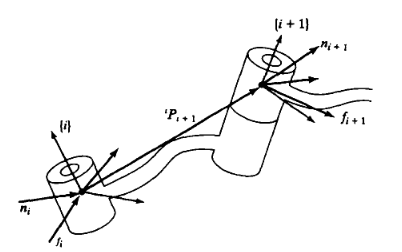
\includegraphics[width=0.5\columnwidth]{imgs/link_forces.png}
\end{figure}

\subsubsection{Calculate the joint Torque required to maintain the static equilibrium}
\paragraph{Rotational joints:} ~\\
Let $^in_i$ be the torque exerted on link $i$ by link $i-1$ relative to link $i$ and\\
let $^i\hat{Z}_i$ be the joint axis vector. \\
The joint torque required to maintain the static equilibrium is computed as:
$$
	\tau_i = ~^in_i^T ⋅ ~^i\hat{Z}_i
$$

\paragraph{Prismatic joints:} ~\\
Let $^if_i$ be the force exerted on link $i$ by link $i-1$ relative to link $i$ and\\
let $^i\hat{Z}_i$ be the joint axis vector. \\
The joint torque required to maintain the static equilibrium is computed as:
$$
\tau_i = ~^if_i^T ⋅ ~^i\hat{Z}_i
$$

\subsection{Jacobians in the Force Domain}
Let $\mathcal{J}$ be a Jacobian (with $\nu  = \mathcal{J}(\Theta)\dot \Theta$) expressed in terms of $\{0\}$ and \\
let $\mathcal{F}$ be a $6 \times 1$ Cartesian force-moment vector acting at the end-effector expressed in terms of $\{0\}$ ($\mathcal{F} = [F, N]^T$ and $F$ is the force acting on the center of the mass of the link and $N$ is the moment acting on the center of the mass of the link)\\
The $6 \times 1$ vector of torques at the joints is calculated as:
$$
	\tau = ~^0\mathcal{J}^T ⋅ ~^0\mathcal{F}
$$

\subsection{Cartesian Transformation of Velocities and static Forces}
Let $^{B}_AR$ a rotation matrix describing $\{A\}$ relative to $\{B\}$ \\
Let $^Av_A$ be the linear velocity of the origin of $\{A\}$ relative to $\{U\}$ expressed in terms of frame $\{A\}$ \\
Let $^A\omega_A$ be the angular velocity vector of $\{A\}$ relative to $\{U\}$ expressed in terms of frame $\{A\}$ \\
Let $^AP_{BORG}$ be the origin of $\{B\}$ relative to $\{A\}$ \\
The vector of Cartesian velocities of $B$ with respect to frame $\{B\}$ is calculated as:
$$
	^B\nu_B = \vect{^Bv_B \\ ^B\omega_B} = \begin{bmatrix}
		^B_AR & -^B_AR ⋅ ~^AP_{BORG}\times \\
		0 & ^B_AR
	\end{bmatrix} \vect{^Av_A \\ ^A\omega_A} = ~^B_AT_v ⋅ ~^A\nu_A
$$
, where
$P\times = \begin{bmatrix}
	0 & -p_z & p_y \\
	p_z & 0 & -p_x \\
	-p_y & p_x & 0
\end{bmatrix}$ and $T_v$ is called a velocity transformation \\
\\

and Let $^{A}_BR$ a rotation matrix describing $\{B\}$ relative to $\{A\}$ \\
It follows:
$$
	^A\nu_A = \vect{^Av_A \\ ^A\omega_A} = \begin{bmatrix}
		^A_BR & ^AP_{BORG} \times ~^A_BR \\
		0 & ^A_BR
	\end{bmatrix} \vect{^Bv_B \\ ^B\omega_B} = ~^A_BT_v ⋅ ~^B\nu_B
$$
\\

and let $^BF_B$ be a force vector and \\
let $^BN_B$ be a moment vector \\
$^A\mathcal{F}_A = \vect{^AF_A \\ ^AN_A}$ is computed as:
$$
	^A\mathcal{F}_A = \vect{^AF_A \\ ^AN_A} = \begin{bmatrix}
		^A_BR & 0 \\
		^AP_{BORG} \times ^A_BR & ^A_BR
	\end{bmatrix} \vect{^BF_B \\ ^BN_B} = ~^A_BT_f ⋅ ~^F\mathcal{F}_B
$$
, where $T_f$ is called a force-moment transformation

\section{Dynamics}
\subsection{Acceleration of a rigid body}
Let $^BV_Q$ the velocity of a point $Q$ relative to $\{B\}$ \\
The linear acceleration of $Q$ relative to $\{B\}$ is defined as:
$$
	^B\dot V_Q = \frac d {dt} ~^BV_Q = \lim_{\Delta t → 0} \frac{^BV_Q(t + \Delta t) - ~^BV_Q(t)}{\Delta t}
$$
\\

Let $^A\Omega_B$ be the angular velocity of a rotation of frame $\{B\}$ relative to $\{A\}$ \\
The angular acceleration of $\{B\}$ relative to $\{A\}$ is defined as:
$$
	^A\dot \Omega_B = \frac d {dt} ~^A\Omega_B = \lim_{\Delta t → 0} \frac{^A\Omega_B(t + \Delta t) - ~^A\Omega_B(t)}{\Delta t}
$$
\\

Let $^UAORG$ be the origin of frame $\{A\}$ relative to frame $\{U\}$ \\
The acceleration of $^UAORG$ relative to the universe frame $\{U\}$ is defined as:
$$
\dot v_A = ~^U\dot V_{AORG}
$$
\\

Let $\{A\}$ be a frame and $\{U\}$ be the universe frame \\
The angular acceleration of a rotation of frame $\{A\}$ relative to $\{U\}$ is defined as:
$$
\dot \omega_A = ~^U \dot \Omega_{A}
$$

\subsubsection{Linear acceleration}
Let $^BQ$ be a position vector relative to frame $\{B\}$ and \\
let $^B\dot V_Q$ be the linear acceleration of $Q$ relative to $\{B\}$ and \\
let $^B V_Q$ be the linear velocity of $Q$ relative to $\{B\}$ and \\
let $^A\dot \Omega_B$ be a vector describing the angular acceleration of $\{B\}$ relative to $\{A\}$ and \\
let $^A\Omega_B$ be a vector describing the angular velocity of $\{B\}$ relative to $\{A\}$ \\
The linear acceleration of a position vector $Q$ relative to $\{A\}$ is calculated as:
$$
	^A\dot V_Q = ~^A\dot{V}_{BORG} + ~^A_BR ⋅ ~^B\dot V_Q + 2 ⋅ ~^A\Omega_B \times ~^A_BR ⋅ ~^BV_Q + ~^A\dot \Omega_B \times ~^A_BR ⋅ ~^BQ + ~^A\Omega_B \times (^A\Omega_B \times ~^A_BR ⋅ ~^BQ)
$$
\\
in the case of $^BV_Q = ^B\dot{V}_Q = 0$:
$$
^A\dot V_Q = ~^A\dot{V}_{BORG} + ~^A\dot \Omega_B \times ~^A_BR ⋅ ~^BQ + ~^A\Omega_B \times (^A\Omega_B \times ~^A_BR ⋅ ~^BQ)
$$

\subsubsection{Angular acceleration}
Let $^A\Omega_B$ be a vector describing the angular velocity of $\{B\}$ relative to $\{A\}$ and \\
let $^A\dot \Omega_B$ be the vector describing the angular acceleration of $\{B\}$ relative to $\{A\}$ and \\
let $^B\Omega_C$ be a vector describing the angular velocity of $\{C\}$ relative to $\{B\}$ and \\
let $^B\dot \Omega_C$ be the vector describing the angular acceleration of $\{C\}$ relative to $\{B\}$ \\
The angular acceleration of a rotation of $\{C\}$ relative to $\{A\}$ is defined as:
$$
	^A\dot \Omega_C = ~^A\dot \Omega_B + ~^A_BR ⋅ ~^B \dot \Omega_C + ~^A\Omega_B \times ~^A_BR ⋅ ~^B\Omega_C
$$

\subsection{Acceleration from link to link}
\subsubsection{Rotational joints}
Let joint $i+1$ be rotational: \\

Let $^i\omega_i$ be the angular velocity vector of link $\{i\}$ relative to $\{B\}$ expressed in terms of frame $\{i\}$ \\
Let $^i\dot\omega_i$ be the angular acceleration vector of link $\{i\}$ relative to $\{B\}$ expressed in terms of frame $\{i\}$ \\
The angular acceleration of link $i + 1$ with respect to frame $\{i + 1\}$ is calculated as:
$$
^{i+1}\dot \omega_{i+1} = ~^{i+1}_iR ⋅ ~^i\dot \omega_i + ~^{i+1}_iR ⋅ ~^i\omega_i \times \dot \theta_{i+1} ⋅ ~^{i+1}\hat{Z}_{i+1} + \ddot \theta_{i+1} ⋅ ~^{i+1}\hat{Z}_{i+1}
$$
, where $\ddot \theta_{i+1} ⋅ ^{i+1}\hat{Z}_{i+1} = ~^{i+1}\vect{0 \\ 0 \\ \ddot{\theta}_{i+1}}$ \\
\\

Let $^i\dot v_i$ be the linear acceleration of the origin of link $\{i\}$ relative to $\{B\}$ expressed in terms of frame $\{i\}$ \\
Let $^i\omega_i$ be the angular velocity vector of link $\{i\}$ relative to $\{B\}$ expressed in terms of frame $\{i\}$ \\
Let $^i\dot \omega_i$ be the angular acceleration vector of link $\{i\}$ relative to $\{B\}$ expressed in terms of frame $\{i\}$ \\
Let $^iP_{i+1}$ be the origin of $\{i+1\}$ relative to $\{i\}$
The linear acceleration of link $i + 1$ with respect to frame $\{i + 1\}$ is calculated as:
$$
^{i+1}\dot v_{i+1} = ~^{i+1}_iR(^i\dot \omega_i \times ~^iP_{i+1} + ~^i\omega_i \times (^i\omega_i \times ~^iP_{i+1}) + ^i\dot v_i)
$$

\subsubsection{Prismatic joints}
Let joint $i+1$ be prismatic: \\

Let $^i\dot \omega_i$ be the angular acceleration vector of link $\{i\}$ relative to $\{B\}$ expressed in terms of frame $\{i\}$ \\
The angular acceleration of link $i + 1$ with respect to frame $\{i + 1\}$ is calculated as:
$$
^{i+1}\dot \omega_{i+1} = ~^{i+1}_iR ⋅ ~^i\dot \omega_i
$$

Let $^iv_i$ be the linear velocity of the origin of link $\{i\}$ relative to $\{B\}$ expressed in terms of frame $\{i\}$ \\
Let $^i\omega_i$ be the angular velocity vector of link $\{i\}$ relative to $\{B\}$ expressed in terms of frame $\{i\}$ \\
Let $^i\dot\omega_i$ be the angular acceleration vector of link $\{i\}$ relative to $\{B\}$ expressed in terms of frame $\{i\}$ \\
Let $^iP_{i+1}$ be the origin of $\{i+1\}$ relative to $\{i\}$
The linear velocity of link $i + 1$ with respect to frame $\{i + 1\}$ is calculated as:
$$
^{i+1}\dot v_{i+1} = ~^{i+1}_iR(~^i\dot \omega_i \times ~^iP_{i+1} + ~^i\omega_i \times (^i \omega_i \times ~^iP_{i+1}) + ~^i\dot v_i) + 2 ⋅ ~^{i+1} \omega_{i+1} \times \dot{d}_{i+1} ⋅ ~^{i+1}\hat{Z}_{i+1} + \ddot{d}_{i+1} ⋅ ~^{i+1}\hat{Z}_{i+1}
$$


\subsection{Mass Distribution}
Let $\rho$ be the density of the material and \\
let the rigid body be composed of differential volume elements $dv$ where each is located with a vector $^AP = [xyz]^T$
The inertia tensor (which can be thought of as a generalization of the scalar moment of inertia of an object) relative to frame $\{A\}$ is defined as:
$$
	^AI = \begin{bmatrix}
		I_{xx} & -I_{xy} & -I_{xz} \\
		-I_{xy} & I_{yy} & -I_{yz} \\
		-I_{xz} & -I_{yz} & -I_{zz} \\
	\end{bmatrix}
$$
, with
$$
	I_{xx} = \int_{} \int_{} \int_V (y^2 + z^2) \rho dv
$$
$$
	I_{yy} = \int_{} \int_{} \int_V (x^2 + z^2) \rho dv
$$
$$
	I_{zz} = \int_{} \int_{} \int_V (x^2 + y^2) \rho dv
$$
$$
	I_{xy} = \int_{} \int_{} \int_V xy \rho dv
$$
$$
	I_{xz} = \int_{} \int_{} \int_V xz \rho dv
$$
$$
	I_{yz} = \int_{} \int_{} \int_V yz \rho dv
$$
\\
The elements $I_{xx}, I_{yy}$ and $I_{zz}$ are called the mass moments of inertia \\
The elements with mixed indices are called the mass products of intertia

\subsubsection{Parallel-axis theorem}
\begin{itemize}
	\item A way of computing how the inertia tensor changes under translations of the reference coordinate system
\end{itemize}

Let $\{C\}$ be located at the center of mass of the body and \\
let $\{A\}$ be an arbitrarily translated frame. \\
The inertia tensor related in a frame with origin at the center of mass to the inertia tensor with respect to another reference frame is defined as:
$$
	^AI_{zz} = ~^CI_{zz} + m(x_c^2 + y_c^2)
$$
$$
	^AI_{xy} = ~^CI_{xy} - mx_cy_c
$$
$$
	^AI = ~^CI + m[P_c^TP_cI_3 - P_cP_c^T]
$$

\subsubsection{Facts about inertia tensors}
\begin{itemize}
	\item If two axes of the reference frame form a plane of symmetry for the mass distribution of the body, the products of inertia having as an index the coordinate that is normal to the plane of symmetry will be zero.
	\item Moments of inertia must always be positive. Products of inertia may have either sign.
	\item The sum of the three moments of inertia is invariant under orientation changes in the reference frame.
	\item The eigenvalues of an inertia tensor are the principal moments for the body. The associated eigenvectors are the principal axes.
	
\end{itemize}


\subsection{Newton's Equation, Euler's Equation}
\subsubsection{Newton's Equation}
Let $m$ be the total mass of a body (e.g. a link) and \\
let $\dot v_C$ be the acceleration with which the center of mass is accelerating. \\
The force acting at the center of mass and causing this acceleration is defined as:
$$
	F = m\dot v_C
$$

\begin{figure}[H]
	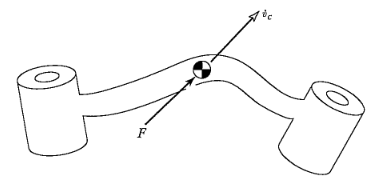
\includegraphics[width=0.5\columnwidth]{imgs/link_newton.png}
\end{figure}

\subsubsection{Euler's Equation}
Let $\omega$ be the angular velocity with which a rigid body is rotating and \\
let $\dot \omega$ be the corresponding acceleration and \\
let $^CI$ be the inertia tensor of the body written in frame $\{C\}$, whose origin is located at the center of mass \\
The moment $N$, which must be acting on the body to cause this motion is defined as:
$$
	N = ~^CI\dot \omega + \omega \times ~^CI \omega
$$

\begin{figure}[H]
	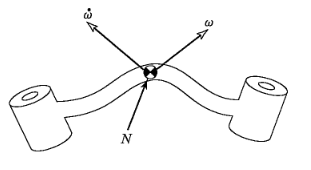
\includegraphics[width=0.5\columnwidth]{imgs/link_euler.png}
\end{figure}

\subsection{Iterative Newton-Euler Dynamic Formulation}
\subsubsection{Outward iterations to compute velocities and acceleration}
Let $\{C_i\}$ be a frame attached to each link, having its origin located at the center of mass of the link and having the same orientation as the link frame $\{i\}$ and \\
let $^i\dot v_i$ be the linear acceleration of the origin of link $\{i\}$ relative to $\{B\}$ expressed in terms of frame $\{i\}$ \\
Let $^i\omega_i$ be the angular velocity vector of link $\{i\}$ relative to $\{B\}$ expressed in terms of frame $\{i\}$ \\
Let $^i\dot \omega_i$ be the angular acceleration vector of link $\{i\}$ relative to $\{B\}$ expressed in terms of frame $\{i\}$ \\
Let $^iP_{C_i}$ be the origin of $\{C_i\}$ relative to $\{i\}$. \\
The linear acceleration of the center of mass of each link is computed as:
$$
	^i\dot v_{C_i} = ~^i \dot \omega_i \times ~^iP_{C_i} + ~^i \omega_i \times (~^i \omega_i \times ~^iP_{C_i}) + ~^i \dot v_i
$$

\subsubsection{Force and Torque acting on a link}
Let $\{C_i\}$ be a frame attached to each link, having its origin located at the center of mass of the link and having the same orientation as the link frame $\{i\}$ and \\
The force and torque acting at the center of mass of each link expressed in $\{i\}$ is computed as:
$$
	^iF_i = m_i ⋅ ~^i\dot v_{C_i}
$$
$$
	^iN_i = ~^{C_i}I_i ⋅ ~^i\dot \omega_i + ~^i\omega_i \times ~^{C_i}I_i ⋅ ~^i\omega_i
$$

\subsubsection{Inward iterations to compute forces and torques}
let $^{i+1}f_{i+1}$ be a force exerted on link $i+1$ by link $i$ relative to link $i+1$ and \\
let $^iF_i$ be the force acting at the center of mass and causing this acceleration relative to $\{i\}$. \\
The force exerted on link $i$ by link $i-1$ relative to link $i$ is defined as:
$$
	^if_i = ~^i_{i+1}R ⋅ ~^{i+1}f_{i+1} + ~^iF_i
$$

Let $^{i+1}n_{i+1}$ be a torque exerted on link $i+1$ by link $i$ relative to link $i+1$ and \\
let $^iP_{i+1}$ be the origin of frame $\{i+1\}$ relative to $\{i\}$ and \\
let $^iP_{C_i}$ be the origin of frame $\{C_i\}$ relative to $\{i\}$ and \\
let $\{C_i\}$ be a frame attached to link $\{i\}$, having its origin located at the center of mass of the link and having the same orientation as the link frame $\{i\}$ and \\
let $^iN_i$ be the torque acting at the center of mass of link $\{i\}$ relative to $\{i\}$ and \\
let $^iF_i$ be the force acting at the center of mass relative to $\{i\}$. \\
The torque exerted on link $i$ by link $i-1$ relative to link $i$ is defined as:
$$
	^in_i = ~^iN_i + ~^i_{i+1}R ⋅ ~^{i+1}n_{i+1} + ~^iP_{C_i} \times ~^iF_i + ~^iP_{i+1} \times ~^i_{i+1}R ⋅ ~^{i+1}f_{i+1}
$$
\\

The required joint torques that will result in the net forces and torques being applied to each link are computed as:
\textbf{Rotational joint:} \\
$$
	\tau_i = ~^in_i^T ⋅ ~^i\hat{Z}_i
$$

\textbf{Prismatic joint:} \\
$$
	\tau_i = ~^if_i^T ⋅ ~^i\hat{Z}_i
$$

\subsubsection{The iterative Newton-Euler dynamics algorithm}
for i = 0 to 5 \\
do \\
\tab	calculate: $^{i+1}\omega_{i+1}$, $^{i+1}\dot \omega_{i+1}$, $^{i+1}\dot v_{i+1}$, $^{i+1}\dot v_{C_{i+1}}$, $^{i+1}F_{i+1}$ and $^{i+1}N_{i+1}$ \\
done \\

for i = 6 downto 1\\ 
do \\
\tab	calculate: $^if_i$, $^in_i$ and $\tau_i$ \\
done \\

\subsubsection{Inclusion of gravity forces in the dynamics algorithm}
Set 
$$
	^0\dot v_0 = G
$$
, where G has the magnitude of the gravity vector but points in the opposite direction 

\subsection{The Structure of a Manipulator's Dynamic Equations}
\subsubsection{State-space Equation}
Let $\tau = [\tau_1, \dots, \tau_n]$ be a vector of actuator torques and \\
let $M(\Theta)$ be the $n \times n$ mass matrix of the manipulator and \\
let $V(\Theta, \dot{\Theta})$ be an $n \times 1$ vector of centrifugal and Coriolis terms and \\
let $G(\Theta)$ be an $n \times 1$ vector of gravity terms. \\
The state-space equation is defined as: \\
$$
	\tau = M(\Theta)\ddot{\Theta} + V(\Theta, \dot{\Theta}) + G(\Theta)
$$

\subsubsection{Configuration-space Equation}
Let $\tau = [\tau_1, \dots, \tau_n]$ be a vector of actuator torques and \\
let $M(\Theta)$ be the $n \times n$ mass matrix of the manipulator and \\
let $B(\Theta)$ be a matrix of dimensions $n \times n(n-1)/2$ of Coriolis coefficient and \\
let $[\dot{\Theta}\dot{\Theta}] = [\dot \theta_1 \dot \theta_2, \dot \theta_1 \dot \theta_3, \dots, \dot \theta_{n-1}\dot \theta_n]^T$ with dimension $n(n-1)/2 \times 1$ and \\
let $C(\Theta)$ be an $n \times n$ matrix of centrifugal coefficients and \\
let $[\dot \Theta^2] = [\dot \theta_1^2, \dots, \dot \theta_n^2]^T$ of dimension $n \times 1$ and \\
let $G(\Theta)$ be an $n \times 1$ vector of gravity terms. \\
The configuration-space equation is defined as: \\
$$
	\tau = M(\Theta)\ddot \Theta + B(\Theta)[\dot \Theta \dot \Theta] + C(\Theta)[\dot \Theta^2] + G(\Theta)
$$

\subsection{Lagrangian Formulation of Manipulator Dynamics}
\subsubsection{Kinematic energy}
Let $m_i$ be the mass of the link $i$ and \\
let $v_{C_i}$ be the linear velocity of the center of mass of link $i$ and \\
Let $^i\omega_i$ be the angular velocity vector of link $\{i\}$ relative to $\{B\}$ expressed in terms of frame $\{i\}$ \\
let $^{C_i}I$ be the inertia tensor of the body written in frame $\{C_i\}$, whose origin is located at the center of mass of link $i$. \\
The kinematic energy of the $i$th link is defined as:
$$
	k_i = \frac 1 2 m_i ⋅ v_{C_i}^T ⋅ v_{C_i} + \frac 1 2 ~^i\omega_i^T ⋅ ~^{C_i}I_i ⋅ ~^i\omega_i
$$

The total kinematic energy of the manipulator is computed as:
$$
	k = \sum_{i = 1}^n k_i
$$
$$
	k(\Theta, \dot \Theta) = \frac 1 2 \dot \Theta^T M(\Theta)\dot \Theta
$$
, where $M(\Theta)$ is the $n \times n$ mass matrix of the manipulator and $\Theta = [\theta_1, \dots, \theta_n]^T$

\subsubsection{Potential energy}
Let $m_i$ be the mass of the link $i$ and \\
let $^0g$ be the $3 \times 1$ gravity vector and \\
let $^0P_{C_i}$ be the vector locating the center of mass of the $i$th link and \\
let $u_{ref_i}$ be a constant chosen so that the minimum values of $u_i$ is zero. \\
The potential energy of the $i$th link is defines as:
$$
	u_i = -m_i ⋅ ~^0g^T ⋅ ~^0P_{C_i} + u_{ref_i}
$$

The total potential energy stored in the manipulator is computed as:
$$
	u = u(\Theta) = \sum_{i = 1}^n u_i
$$

\subsubsection{Lagrangian formulation}
Let $k(\Theta, \dot \Theta)$ be the total kinematic energy of a manipulator and \\
let $u(\Theta)$ be the total potential energy of the manipulator. \\
The Lagrangian of the manipulator is:
$$
	\mathcal{L}(\Theta, \dot \Theta) = k(\Theta, \dot \Theta) - u(\Theta)
$$

The equations of motions for the manipulator are given by:
$$
	\frac d {dt} \frac {\partial k(\Theta, \dot \Theta)}{\partial \dot \Theta} - \frac {\partial k(\Theta, \dot \Theta)}{\partial \Theta} + \frac {\partial u(\Theta)}{\partial \Theta} = \tau
$$

\subsection{Formulating Manipulator Dynamics in Cartesian Space}
\subsubsection{Cartesian state-space equation}
Let $\mathcal{J}(\Theta)$ be the Jacobian with $\tau = \mathcal{J}^T(\Theta)\mathcal{F}$ and \\
let $M(\Theta)$ be the $n \times n$ mass matrix of the manipulator and \\
let $V(\Theta, \dot{\Theta})$ be an $n \times 1$ vector of centrifugal and Coriolis terms and \\
let $G(\Theta)$ be an $n \times 1$ vector of gravity terms. \\

The Cartesian mass matrix of the manipulator is defined as:
$$
	M_X(\Theta) = \mathcal{J}^{-T}(\Theta)M(\Theta)\mathcal{J}^{-1}(\Theta)
$$

The Vector of velocity terms in Cartesian space is defines as:
$$
	V_X(\Theta, \dot \Theta) = \mathcal{J}^{-T}(\Theta)(V(\Theta, \dot \Theta) - M(\Theta)\mathcal{J}^{-1}(\Theta)\dot{\mathcal{J}}(\Theta)\dot \Theta)
$$

The vector of gravity terms in Cartesian space is defined as:
$$
	G_X(\Theta) = \mathcal{J}^{-T}(\Theta)G(\Theta)
$$

The force-torque vector is defined as:
$$
	\mathcal{F} = M_X(\Theta) \ddot \chi + V_X(\Theta, \dot \Theta) + G_X(\Theta)
$$
, where $\ddot{\chi} = \dot{\mathcal{J}} \dot \Theta + \mathcal{J} \ddot \Theta$

\subsubsection{Cartesian configuration space torque equation}
Let $\tau = [\tau_1, \dots, \tau_n]$ be a vector of actuator torques and \\
let $M_X(\Theta)$ be the $n \times n$ Cartesian mass matrix of the manipulator and \\
let $B_X(\Theta)$ be a matrix of dimensions $n \times n(n-1)/2$ of Coriolis coefficient and \\
let $[\dot{\Theta}\dot{\Theta}] = [\dot \theta_1 \dot \theta_2, \dot \theta_1 \dot \theta_3, \dots, \dot \theta_{n-1}\dot \theta_n]^T$ with dimension $n(n-1)/2 \times 1$ and \\
let $C_X(\Theta)$ be an $n \times n$ matrix of centrifugal coefficients and \\
let $[\dot \Theta^2] = [\dot \theta_1^2, \dots, \dot \theta_n^2]^T$ of dimension $n \times 1$ and \\
let $G(\Theta)$ be an $n \times 1$ vector of gravity terms. \\
The configuration-space equation is defined as: \\
$$
	\tau = \mathcal{J}^T(\Theta)M_X(\Theta)\ddot{\chi} + B_X(\Theta)[\dot \Theta \dot \Theta] + C_X(\Theta)[\dot \Theta^2] + G(\Theta)
$$
, where in general $B_X(\Theta) ≠ B(\Theta)$ and $C_X(\Theta) ≠ C(\Theta)$

\subsection{Inclusion of Nonrigid Body Effects}
The viscous friction is defined as:
$$
	\tau_{friction} = v \dot \theta
$$

The Coulomb-friction is defined as:
$$
	\tau_{friction} = c ⋅ \textrm{sgn}(\dot \theta)
$$
, where $c$ is a Coulomb-friction constant

The viscous and Coulomb friction is defined as:
$$
f(\theta, \dot \theta) = \tau_{friction} = c ⋅ \textrm{sgn}(\dot \theta) + v \dot \theta
$$

The state-space equation with inclusion of friction is defined as: \\
$$
\tau = M(\Theta)\ddot{\Theta} + V(\Theta, \dot{\Theta}) + G(\Theta) + F(\Theta, \dot \Theta)
$$


\section{Trajectory Generation}
\begin{itemize}
	\item \textbf{Trajectory:} a time history of position, velocity and acceleration for each degree of freedom
	\item \textbf{Path-update rate:} the rate, the trajectory points are computed (typically 60 Hz - 2000 Hz)
	\item \textbf{Motions of a manipulator:} motions of the tool frame $\{T\}$ relative to the station frame $\{S\}$
	\item \textbf{Via points:} intermediate frames between the initial and final position
	\item \textbf{Path points:} includes all the via points plus the initial and final points (Here: points are frames)
\end{itemize}

\subsection{Joint-Space Schemes}
\begin{itemize}
	\item methods of path generation in which the path shapes (in space and time) are described in terms of function of joint angles
	\item $\theta$ describes the joint angle, $\dot{\theta}$ the velocity and $\ddot{\theta}$ the acceleration
\end{itemize}

\subsubsection{Cubic polynomials}
\begin{itemize}
	\item Smooth function
	\item Velocity at initial and goal position is 0
\end{itemize}
Let $\theta$ be the a joint angle and \\
let $\theta_0$ the angle of the initial position and \\
let $\theta_f$ the angle of the goal position and \\
let $\theta(t)$ be a function that describes the angle relative to the time $t$ where $\theta(t_0)$ is the initial position and $\theta(t_f)$ is the goal position. \\
It follows: \\
$$
	\theta(t_0 = 0) = \theta_0
$$
$$
	\theta(t_f) = \theta_f
$$
$$
	\dot{\theta}(0) = 0
$$
$$
	\dot{\theta}(t_f) = 0
$$
$$
	\theta(t) = \theta_0 + \left(\frac{3}{t_f^2}(\theta_f - \theta_0)\right) ⋅ t^2 + \left(-\frac{2}{t_f^3}(\theta_f - \theta_0)\right) ⋅ t^3
$$
$$
	\dot{\theta}(t) = \left(\frac{6}{t_f^2}(\theta_f - \theta_0)\right) ⋅ t + \left(-\frac{6}{t_f^3}(\theta_f - \theta_0)\right) ⋅ t^2
$$
$$
	\ddot{\theta}(t) = \left(\frac{6}{t_f^2}(\theta_f - \theta_0)\right) + \left(-\frac{12}{t_f^3}(\theta_f - \theta_0)\right) ⋅ t
$$

\subsubsection{Cubic polynomials for a path with via points}
\begin{itemize}
	\item Velocity at initial and goal position is ≥ 0
\end{itemize}
Let $\theta$ be the a joint angle with $\theta_0$ the angle of the position of the via point and $\theta_f$ the angle of the position of the next via point. \\
Let $\theta(t)$ be a function that describes the angle relative to the time $t$ where $\theta(t_0)$ is the position of the via point and $\theta(t_f)$ is the position of the next via point. It follows: \\
$$
	\theta(t_0 = 0) = \theta_0
$$
$$
	\theta(t_f) = \theta_f
$$
$$
	\dot{\theta}(0) = \dot{\theta}_0
$$
$$
	\dot{\theta}(t_f) = \dot{\theta}_f
$$
$$
\theta(t) = \theta_0 + \dot{\theta}_0 ⋅ t + \left(\frac{3}{t_f^2}(\theta_f - \theta_0)-\frac{2}{t_f} \dot{\theta}_0 - \frac{1}{t_f}\dot{\theta}_f \right) ⋅ t^2 + \left(-\frac{2}{t_f^3}(\theta_f - \theta_0) + \frac{1}{t_f^2} (\dot{\theta}_f + \dot{\theta}_0) \right) ⋅ t^3
$$
$$
\dot{\theta}(t) = \dot{\theta}_0 + \left(\frac{6}{t_f^2}(\theta_f - \theta_0) - \frac{4}{t_f} \dot{\theta}_0 - \frac{2}{t_f}\dot{\theta}_f \right) ⋅ t + \left(-\frac{6}{t_f^3}(\theta_f - \theta_0) + \frac{3}{t_f^2} (\dot{\theta}_f + \dot{\theta}_0) \right) ⋅ t^2
$$
$$
\ddot{\theta}(t) =\left(\frac{6}{t_f^2}(\theta_f - \theta_0) - \frac{4}{t_f} \dot{\theta}_0 - \frac{2}{t_f}\dot{\theta}_f \right) + \left(-\frac{12}{t_f^3}(\theta_f - \theta_0) + \frac{6}{t_f^2} (\dot{\theta}_f + \dot{\theta}_0) \right) ⋅ t^2
$$

\subsubsection{High-order polynomials}
\begin{itemize}
	\item Smooth function
	\item Velocity at initial and goal position is ≥ 0
	\item Acceleration at initial and goal position is specified
\end{itemize}
Let $\theta$ be the a joint angle, and \\
let $\theta_0$ be the angle of the initial position, and \\
let $\theta_f$ be the angle of the goal position, and \\
let $\theta(t)$ be a function that describes the angle relative to the time $t$, and \\
let $\theta(t_0)$ be the initial position, and \\
let $\theta(t_f)$ be the goal position. \\
It follows: \\
$$
\theta(t_0 = 0) = \theta_0
$$
$$
\theta(t_f) = \theta_f
$$
$$
\dot{\theta}(0) = \dot{\theta}_0
$$
$$
\dot{\theta}(t_f) = \dot{\theta}_f
$$
$$
\ddot{\theta}(0) = \ddot{\theta}_0
$$
$$
\ddot{\theta}(t_f) = \ddot{\theta}_f
$$
$$
\begin{multlined}
\theta(t) = \theta_0 + \dot{\theta}_0 ⋅ t + \frac{\ddot{\theta}_0}{2} ⋅ t^2 + \frac{20\theta_f - 20\theta_0 - (8\dot{\theta}_f + 12\dot{\theta}_0)t_f - (3\ddot{\theta}_0 - \ddot{\theta}_f)t_f^2}{2 t_f^3} ⋅ t^3 \\ + \frac{30\theta_0 - 30\theta_f + (14\dot{\theta}_f + 16\dot{\theta}_0)t_f + (3\ddot{\theta}_0 - 2\ddot{\theta}_f)t_f^2}{2 t_f^4} ⋅ t^4 + \frac{12\theta_f - 12\theta_0 - (6\dot{\theta}_f + 6\dot{\theta}_0)t_f - (\ddot{\theta}_0 - \ddot{\theta}_f)t_f^2}{2 t_f^5} ⋅ t^5
\end{multlined}
$$

\subsubsection{Linear function with parabolic blends}
\begin{itemize}
	\item Linear function with smooth start and end (parabolic blends)
\end{itemize}
Let $\theta_0$ be the angle of the initial position and \\
let $\theta_f$ be the angle of the goal position. \\
The time at the end of the blend region is computed as:
$$
	t_b = \frac t 2 - \frac{\sqrt{\ddot{\theta}^2t^2 - 4\ddot{\theta}(\theta_f - \theta_0)}}{2\ddot{\theta}}
$$
, where
$$
	\ddot{\theta} ≥ \frac{4(\theta_f - \theta_0)}{t^2}
$$
\\

The value of $\theta$ at the end of the blend region is computed as:
$$
	\theta_b = \theta_0 + \frac 1 2 \ddot \theta t_b^2
$$
\\

\begin{itemize}
	\item $\ddot{\theta} \textbf{ = } \frac{4(\theta_f - \theta_0)}{t^2}$ $\implies$ the linear portion  length is 0 and the path is composed of two blends that connect
	\item $\ddot{\theta} → ∞$ $\implies$ the length of the blend region $→ 0$
\end{itemize}

\subsubsection{Linear function with parabolic blends for a path with via points}
Let $j,k,l$ be 3 neighboring path points and \\
let the duration of the blend region at path point $k$ be $t_k$ and \\
let the duration of the linear portion between $j$ and $k$ be $t_{jk}$ and \\
let the overall duration of the segment connecting $j$ and $k$ be $t_{djk}$ and \\
let the velocity during the linear portion be $\dot{\theta}_{jk}$ and \\
let the acceleration during the blend at point $j$ be $\ddot{\theta}_j$ and \\
let the angle at the path point $k$ be $\theta_k$ \\
It follows:
$$
	\dot{\theta}_{jk} = \frac{\theta_k - \theta_j}{t_{djk}}
$$
$$
	\ddot{\theta}_k = \textrm{sgn}(\dot{\theta}_{kl} - \dot{\theta}_{jk})|\ddot{\theta}_k|
$$
$$
	t_k = \frac{\dot{\theta}_{kl} - \dot{\theta}_{jk}}{\ddot{\theta}_k}
$$
$$
	t_{jk} = t_{djk} - \frac 1 2 t_j - \frac 1 2 t_k
$$
\\

Let $1$ be the initial path point \\
It follows: \\
$$
	\ddot{\theta}_1 = \textrm{sgn}(\theta_2 - \theta_1)|\ddot{\theta}_1|
$$
$$
	t_1 = t_{d12} - \sqrt{t_{d12}^2 - \frac{2(\theta_2 - \theta_1)}{\ddot{\theta}_1}}
$$
$$
	\dot{\theta}_{12} = \frac{\theta_2 - \theta_1}{t_{d12} - \frac 1 2 t_1}
$$
$$
	t_{12} = t_{d12} - t_1 - \frac 1 2 t_2
$$

Let $n$ be the final path point \\
It follows: \\
$$
\ddot{\theta}_n = \textrm{sgn}(\theta_{n-1} - \theta_n)|\ddot{\theta}_n|
$$
$$
t_n = t_{d(n-1)n} - \sqrt{t_{d(n-1)n}^2 - \frac{2(\theta_n - \theta_{n-1})}{\ddot{\theta}_n}}
$$
$$
\dot{\theta}_{(n-1)n} = \frac{\theta_n - \theta_{n-1}}{t_{d(n-1)n} - \frac 1 2 t_n}
$$
$$
t_{(n-1)n} = t_{d(n-1)n} - t_n - \frac 1 2 t_{n-1}
$$

\begin{figure}[H]
	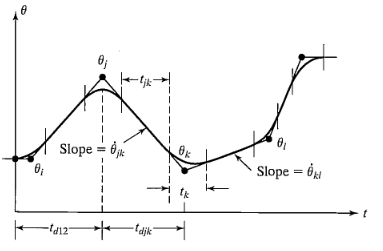
\includegraphics[width=0.5\columnwidth]{imgs/trajectory_via.png}
\end{figure}

\subsection{Cartesian-Space Schemes}
\subsubsection{Geometric Problems with Cartesian Paths}
\begin{itemize}
	\item \textbf{Intermediate points unreachable:} It is possible that some points lying on the path are outside of the workspace.
	\item \textbf{High joint rates near singularity:} If a manipulator is following a Cartesian straight-line path and approaches a singular configuration of the mechanism, one or more joint velocities might increase toward infinity. Because velocities of the mechanism are upper bounded, this situation usually results in the manipulator's deviating from the desired path.
	\item \textbf{Start and Goal reachable in different solutions:} The goal point cannot be reached in the same physical solution as the robot is at the start point.
\end{itemize}

\subsection{Path Generation at Runtime}
\subsubsection{Generation of joint-space paths}
\paragraph{Linear Splines with Parabolic blends} ~\\
\textbf{In the linear portion:} \\
$$
	\theta = \theta_j + \dot{\theta}_{jk}t
$$
$$
	\dot{\theta} = \dot{\theta}_{jk}
$$
$$
	\ddot{\theta} = 0
$$
, where $t$ is the time since the $j$th via point

\textbf{In the blend region:} \\
$$
	t_{inb} = t - (\frac 1 2 t_j + t_{jk})
$$
$$
	\theta = \theta_j + \dot \theta_{jk}(t - t_{inb}) + \frac 1 2 \ddot \theta_k t_{inb}^2
$$
$$
	\dot \theta = \dot \theta_{jk} + \ddot \theta_k t_{inb}
$$
$$
	\ddot \theta = \ddot \theta_k
$$
, where t is being reset to $\frac 1 2 t_k$ when a linear segment is entered

\section{Manipulator-mechanism design}
\subsection{Elements of a Robot System}
\begin{itemize}
	\item The manipulator, including its internal or proprioceptive sensors
	\item The end-effector, or end-of-arm tooling
	\item External sensors and effectors, such as vision systems and part feeders
	\item The controller.	
\end{itemize}

\subsection{Steps}
\begin{itemize}
	\item Choose general kinematic structure
	\item Choose actuation (Actuator, Reduction, Transmission)
	\item Select sensors
\end{itemize}

\subsection{Task Requirements}
\begin{itemize}
	\item \textbf{Number of degrees of freedom:} The number of degrees of freedom in a manipulator should match the number required by the task
	\item \textbf{Workspace}
	\item \textbf{Load capacity:} Depends upon the sizing of its structural members, power-transmission system and actuators
	\item \textbf{Speed:} High speed offers advantages in many applications; For some applications the process itself limits the speed rather than the manipulator
	\item \textbf{Repeatability and accuracy:} High repeatability and accuracy are expensive to achieve
\end{itemize}

\subsection{Kinematic configuration}
\textbf{Often used kinematic design:}
\begin{itemize}
	\item \textbf{Position structure:} Position the wrist (first 3 joints)
	\item \textbf{Orienting structure/Wrist:} Orient the end-effector and have axes that intersect at the wrist point (last 3 joints)
\end{itemize}

\subsubsection{Cartesian}
\begin{itemize}
	\item Structure:	
	\begin{itemize}
		\item First 3 joints are prismatic, mutually orthogonal and correspond to the $\hat{X}, \hat{Y}$ and $\hat{Z}$ Cartesian directions
	\end{itemize}
	\item Often used for gantry robots
\end{itemize}

\begin{figure}[H]
	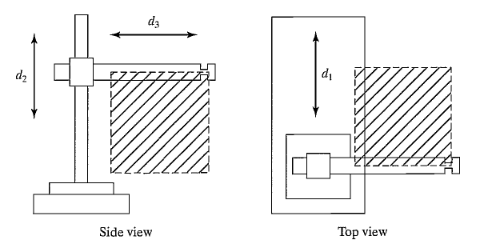
\includegraphics[width=0.5\columnwidth]{imgs/man_cartesian.png}
\end{figure}

\subsubsection{Articulated}
\begin{itemize}
	\item Structure:	
	\begin{itemize}
		\item 2 "shoulder" joints (one for rotation about a vertical axis and one for elevation out of the horizontal plane)
		\item 1 "elbow" joint (usually parallel to the shoulder joint)
		\item 2 or 3 wrist joints at the end of the manipulator
	\end{itemize}
	\item Also called jointed, elbow or anthropomorphic manipulator
\end{itemize}

\begin{figure}[H]
	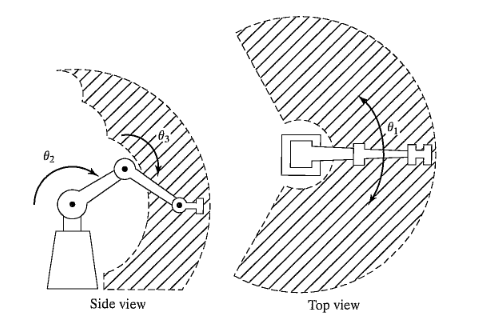
\includegraphics[width=0.5\columnwidth]{imgs/man_articulated.png}
\end{figure}

\subsubsection{SCARA}
\begin{itemize}
	\item Structure:
	\begin{itemize}
		\item 3 parallel revolute joints (for moving and orient in a plane)
		\item 1 prismatic joint (for moving the end effector normal to the plane)
	\end{itemize}
	\item First 3 joints don't have to support any of the weight of the manipulator or the load
	\item Link 0 can house the actuators for the first 2 joints
	\item Can move very fast
\end{itemize}

\begin{figure}[H]
	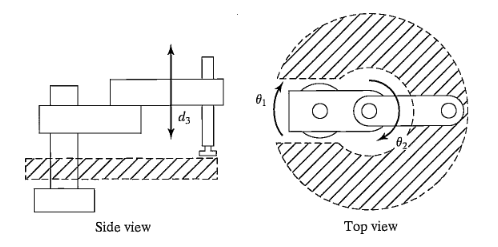
\includegraphics[width=0.5\columnwidth]{imgs/man_scara.png}
\end{figure}

\subsubsection{Spherical}
\begin{itemize}
	\item Structure:
	\begin{itemize}
		\item 2 "shoulder" joints (one for rotation about a vertical axis and one for elevation out of the horizontal plane)
		\item 1 prismatic joint
		\item may (2 or 3 wrist joints at the end of the manipulator)
	\end{itemize}
\end{itemize}

\begin{figure}[H]
	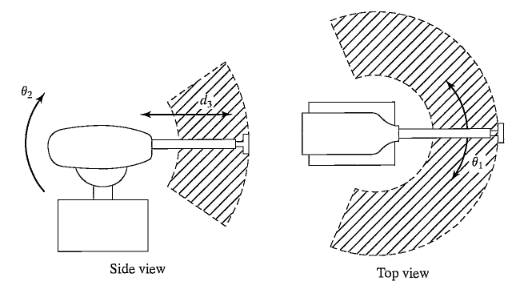
\includegraphics[width=0.5\columnwidth]{imgs/man_spherical.png}
\end{figure}

\subsubsection{Cylindrical}
\begin{itemize}
	\item Structure:
	\begin{itemize}
		\item 1 revolute joint (with a vertical axis)
		\item 1 prismatic joint (for translating vertically)
		\item 1 prismatic joint (for translating horizontally)
	\end{itemize}
\end{itemize}

\begin{figure}[H]
	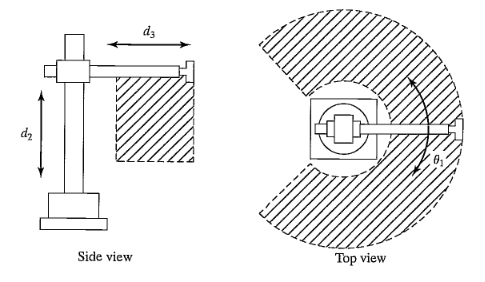
\includegraphics[width=0.5\columnwidth]{imgs/man_cylindrical.png}
\end{figure}

\subsubsection{Wrist}
\paragraph{Most common wrist configuration} ~\\
\begin{itemize}
	\item Structure:
	\begin{itemize}
		\item 2 or 3 revolute joints with orthogonal intersecting axes
	\end{itemize}
	\item Any orientation can be reached
	\item Closed-form kinematic solution exist
\end{itemize}

\begin{figure}[H]
	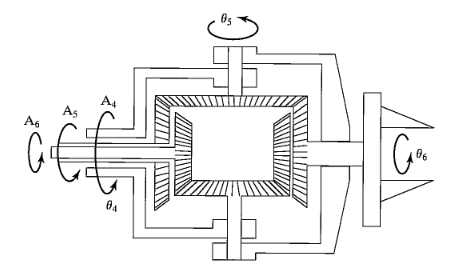
\includegraphics[width=0.5\columnwidth]{imgs/wrist_orthogonal.png}
\end{figure}

\paragraph{Parallel joints} ~\\
\begin{itemize}
	\item Structure:
	\begin{itemize}
		\item joint-2, joint-3 and joint-4 axes are parallel
	\end{itemize}
	\item Closed-form kinematic solution exist
\end{itemize}

\begin{figure}[H]
	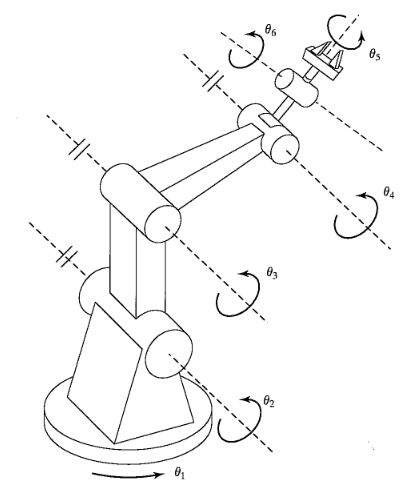
\includegraphics[width=0.5\columnwidth]{imgs/wrist_parallel.png}
\end{figure}

\paragraph{5-DOF welding robot} ~\\
\begin{itemize}
	\item Structure:
	\begin{itemize}
		\item 2 revolute joints with orthogonal intersecting axes
	\end{itemize}
\end{itemize}

\begin{figure}[H]
	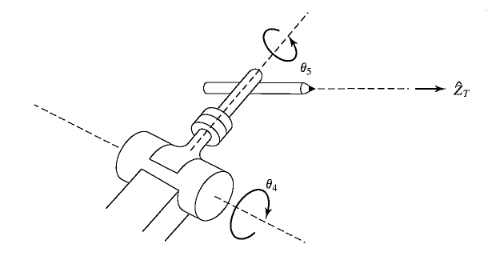
\includegraphics[width=0.5\columnwidth]{imgs/wrist_welding.png}
\end{figure}

\subsection{Quantitative Measures of Workspace Attributes}
\subsubsection{Efficiency of design in terms of generating workspace}
Let $a_i-1$ be the link length of link $i-1$ and \\
let $d_i$ be the link offset of joint $i$ and \\
let $N$ be the number of joints. \\
The length sum of a manipulator is computed as:
$$
	L = \sum_{i = 1}^N(a_{i-1} + d_i)
$$
\\

Let $L$ be the length sum of a manipulator and \\
let $W$ be the volume of the manipulator's workspace \\
The structural length index is defined as:
$$
	Q_L = \frac{L}{\sqrt[3]{W}}
$$
, where good designs have a low $Q_L$

\subsubsection{Designing well-conditioned workspaces}
\begin{itemize}
	\item When the manipulator is near a singular point, actions of the manipulator are said to be poorly conditioned
\end{itemize}
Let $\mathcal{J}(\Theta)$ be the Jacobian of a manipulator. \\
The manipulability measure is defined as:
$$
	w = \sqrt{\det(\mathcal{J}(\Theta)\mathcal{J}^T(\Theta)}
$$
\\

The manipulability measure for a nonredundant manipulator is defined as:
$$
	w = |\det(\mathcal{J}(\Theta))|
$$
, where good designs have high values of $w$ \\
\\

Let $M(\Theta)$ be the mass matrix of the manipulator and \\
let $M_X(\Theta)$ be the Cartesian mass matrix of the manipulator and \\
let $\mathcal{J}(\Theta)$ be the Jacobian of a manipulator. \\
The manipulability measure based on acceleration analysis or force-application capability is defined as:
$$
	M_X(\Theta) = \mathcal{J}^{-T}(\Theta)M(\Theta)\mathcal{J}^{-1}(\Theta)
$$

\subsection{Redundant and Closed-Chain Structures}
\subsubsection{Micromanipulators and other redundancies}
\begin{itemize}
	\item Avoidance of singular configurations
	\item Avoidance of collisions while operating in cluttered work environments
\end{itemize}

\subsubsection{Closed-loop structures}
\begin{itemize}
	\item Structure with parallel links
	\item Increase the stiffness of the mechanism
	\item Reduces the allowable range of motion of the joints and thus decrease the workspace size
\end{itemize}

Let $l$ be the number of links (including the base) and \\
let $n$ be the total number of joints and \\
let $f_i$ be the number of degrees of freedom associated with the $i$th joint. \\
The Grübler's formula which computes the total number of degrees of freedom is defined as
$$
	F = 6(l - n - 1) + \sum_{i = 1}^n f_i
$$

\subsection{Actuation Schemes}
\subsubsection{Actuator location}
\begin{itemize}
	\item \textbf{Direct-drive}
	\begin{itemize}
		\item Placed at the joint
		\item Simple in design
		\item High controllability
		\item No transmission or reduction elements
	\end{itemize}
	\item \textbf{Speed-reduction system}
	\begin{itemize}
		\item Many actuators are suited to high speeds and low torques
		\item Could be placed either at the actuator or at the joint
		\item Lowers speed and increases the torque
		\item Adds complexity, friction and flexibility
	\end{itemize}
	\item \textbf{Transmission system}
		\item Actuators tend to be rather heavy. By locating them from the joint to the base, the overall inertia can be reduced.
		\item Transfers the motion from the actuator to the joint
		\item Adds complexity, friction and flexibility
\end{itemize}

\subsubsection{Reduction and transmission systems}
\begin{itemize}
	\item \textbf{Gears}
	\begin{itemize}
		\item Most common element used for reduction
		\item Can produce large reduction in compact configurations
		\item But adds backlash and friction
	\end{itemize}
	\item \textbf{Cables, flexible bands, belts, roller chains}
	\begin{itemize}
		\item Able to combine transmission with reduction
	\end{itemize}
	\item \textbf{Lead screws (a), ball-bearing screws (b)}
	\begin{itemize}
		\item Are very stiff
		\item Can support very large loads
		\item Able to transform rotary motion into linear motion
		\item Ball-bearing screwa have very low friction
	\end{itemize}
\end{itemize}

\begin{figure}[H]
	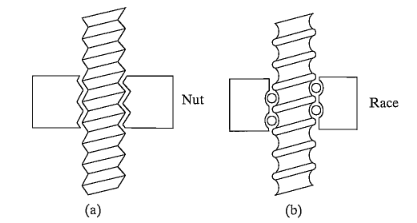
\includegraphics[width=0.5\columnwidth]{imgs/lead_screws.png}
\end{figure}

\paragraph{Gear ratio} ~\\
Let $\eta$ be speed-reducing and torque-increasing effect of a gear pair ($\eta > 1$) and \\
let $\dot \theta_i$ be the input speed. \\
The output speed is calculated as:
$$
	\dot \theta_o = \frac {\dot \theta_i} \eta 
$$
\\
Let $\eta$ be speed-reducing and torque-increasing effect of a gear pair ($\eta > 1$) and \\
let $\tau_i$ be the input torque. \\
The output torque is calculated as:
$$
	\tau_o = \eta\tau_i
$$

Let $r2$ be the radius of the output pulley(using bends, cables, \dots)/gear and \\
let $r1$ be the radius of the input pulley/gear. \\
The gear ratio is defined as:
$$
	\eta = \frac{r_2}{r_1}
$$

\begin{figure}[H]
	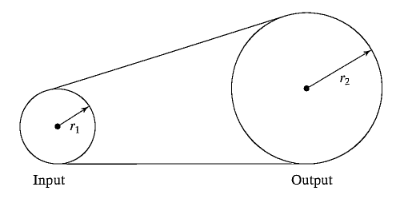
\includegraphics[width=0.5\columnwidth]{imgs/pulleys.png}
\end{figure}

\subsection{Stiffness and Deflections}
\subsubsection{Flexible elements in parallel and in series}
Let $k_1$ and $k_2$ the stiffness of 2 flexible members connected in parallel. \\
The produced net stiffness is calculated as:
$$
	k_{parallel} = k_1 + k_2
$$
\\

Let $k_1$ and $k_2$ the stiffness of 2 flexible members connected in series. \\
The produced net stiffness is calculated as:
$$
	\frac{1}{k_{series}} = \frac{1}{k_1} + \frac{1}{k_2}
$$

\subsubsection{Shafts}
Let $G$ be the shear modulus of elasticity (e.g. $7.5 \times 10^{10} Nt/m^2$ for steel) and \\
let $d$ be the shaft diameter and \\
let $l$ be the shaft length. \\
Th torsional stiffness of a round shaft can be calculated as:
$$
	k = \frac{G\pi d^4}{32l}
$$

\subsubsection{Gears}
Let $C_g = 1.34 \times 10^{10} Nt/m^2$ for steel and \\
let $b$ be the face width of the gears and \\
let $r$ be the radius of the output gear. \\
The stiffness of the output gear is calculated as:
$$
	k = C_gbr^2
$$
\\

Let $\eta$ be the gear ratio and \\
let $k_i$ be the stiffness of the input gear. \\
The stiffness of the output gear is computed as:
$$
	k_o = \frac{\tau_o}{\delta\theta_o} = \frac{\eta k_i \delta \theta_i}{\frac 1 \eta \delta \theta_i} = \eta^2 k_i
$$

\subsubsection{Belts}
Let $A$ be the cross-sectional area of the belt and \\
let $E$ be the modulus of elasticity of the belt and \\
let $l$ be the length of the free belt between pulleys + $\frac 1 3$ of the length of the belt in contact  with the pulleys. \\
The stiffness of the belt drive is calculated as:
$$
	k = \frac{AE}{l}
$$

\subsubsection{Links}
Let $E$ be the modulus of elasticity (e.g. $2 \times 10^{11} Nt/m^2$ for steel) and \\
let $d_i$ and $d_o$ be the inner and outer diameters of the tubular beam and \\
let $w_i$ and $w_o$ be the inner and outer widths of the beam (i.e. wall thickness is $(w_o - w_i)/2$) and \\
let $l$ be the length. \\

The stiffness of a round hollow beam is computed as:
$$
	k = \frac{3 \pi E (d_o^4 - d_i^4)}{64 l^3}
$$

The stiffness of a square-cross-section hollow beam is computed as:
$$
	k = \frac{E (w_o^4 - w_i^4)}{4l^3}
$$

\subsection{Actuators}
\subsubsection{Hydraulic cylinders}
\begin{itemize}
	\item High forces; No need of a reduction system
	\item Speed depends upon the pump and accumulator system
	\item Position control is well understood and straightforward
	\item Require a lot of equipment (pumps, accumulators, hoses, servo valves)
	\item Tend to be inherently messy
\end{itemize}

\subsubsection{Pneumatic cylinders}
\begin{itemize}
	\item High forces; No need of a reduction system
	\item Speed depends upon the pump and accumulator system
	\item Cleaner than hydraulics
	\item Difficult to control accurately
\end{itemize}

\subsubsection{Brush motors}
\begin{itemize}
	\item High peak torques but only much lower torques over long periods of time
	\item windings gain high temperature
	\item Problems of Brush wear and friction
\end{itemize}

\subsubsection{Brushless motors}
\begin{itemize}
	\item No brush wear and friction
	\item Possibility to attach the windings outside to the motor case → Better cooling
\end{itemize}

\subsection{Position Sensing}
\subsubsection{Rotary Optical Encoder}
\begin{itemize}
	\item As the encoder shaft turns, a disk containing a pattern of fine lines interrupts a light beam. The shaft angle is determined by counting the number of pulses.
	\item To determine the direction, there are two such channels, with wave pulse trains 90 degrees out of phase. The direction of rotation is determined by the relative phase of the two square waves
\end{itemize}

\subsubsection{Resolvers}
\begin{itemize}
	\item Devices that output 2 signals (the sine of the shaft angel and the the cosine)
	\item The shaft angle is computed from the relative magnitude of the two signals
	\item Often more reliable than optical encoders
	\item Lower resolution than optical encoders
\end{itemize}

\subsubsection{Potentiometers}
\begin{itemize}
	\item Produce a voltage proportional to the shaft position
	\item Limited by resolution, linearity and noise susceptibility
\end{itemize}

\subsubsection{Tachometers}
\begin{itemize}
	\item Provide an analog signal proportional to the shaft velocity
\end{itemize}

\subsection{Force Sensing}
\subsubsection{Placements of Force sensors}
\begin{itemize}
	\item \textbf{At the joint actuators:} measure the torque/force output of the actuator itself
	\item \textbf{Between the end-effector and the last joint of the manipulator:} referred to as wrist sensors; measures the force/torques acting on the end-effector
	\item \textbf{At the fingertips:} measure from one to four components of force acting at each fingertip
\end{itemize}


\section{Linear control of manipulators}
\begin{itemize}
	\item the system can be modeled mathematically by linear differential equations
\end{itemize}

\subsection{Feedback and Closed-loop Control}
\subsubsection{Open-loop scheme}
\begin{itemize}
	\item Calculation of the torques for the actuators without made of use of the feedback from the sensors (position, velocity sensors)
\end{itemize}

\subsubsection{Closed-loop scheme}
\begin{itemize}
	\item Calculation of the torques for the actuators with made of use of the feedback from the sensors (position, velocity sensors)
	\item A bad designed control system can result in unstable performance (Servo Error increasing instead of decreasing)
\end{itemize}

\begin{figure}[H]
	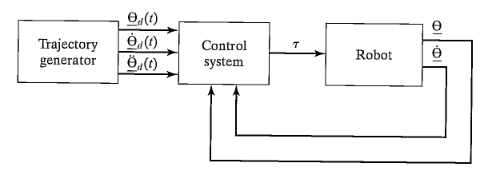
\includegraphics[width=0.5\columnwidth]{imgs/closed_loop_scheme.png}
\end{figure}

\subsubsection{Servo Error}
\begin{itemize}
	\item Presence of disturbances (noise) leads to deviant position
\end{itemize}
Let $\Theta_d$ and $\dot \Theta_d$ be the desired position and velocity of the trajectory and \\
let $\Theta$ and $\dot \Theta$ be actual position and velocity. \\
The difference between the desired and the actual position is computed as: 
$$
	E = \Theta_d - \Theta
$$
The difference between the desired and the actual velocity is computed as: 
$$
	\dot E = \dot \Theta_d - \dot \Theta
$$

\subsubsection{Independent Joint Control}
\begin{itemize}
	\item Uses an independent single-input, single-output (SISO) control system for each joint
	\item Adopted by most industrial robot suppliers
\end{itemize}

\subsection{Second-Order Linear Systems}
\begin{figure}[H]
	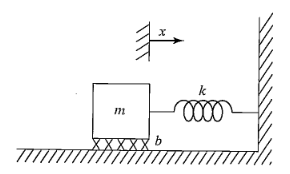
\includegraphics[width=0.5\columnwidth]{imgs/spring_mass.png}
\end{figure}

Let be given a spring-mass system with friction where \\
$m$ be the mass of a block attached to the spring and \\
$k$ be the stiffness of the spring and \\
$b$ a coefficient of friction. \\
It follows:
$$
	m\ddot x + b \dot x + k x = 0
$$
\\

The corresponding characteristic equation is defined as:
$$
	ms^2 + bs + k = 0
$$
with the roots (poles of the system)
$$
	s_{1,2} = - \frac{b}{2m} \pm \frac{\sqrt{b^2 - 4mk}}{2m}
$$

\subsubsection{Real and Unequal Roots}
\begin{itemize}
	\item If the roots are real and negative → Overdamped (non-oscillatory exponential decay)
	\item If the roots are real and positive → Not BIBO stable (non-oscillatory exponential increase)
\end{itemize}
~\\

Let $b^2 > 4mk$ \\
It follows:
$$
	x(t) = c_1e^{s_1t} + c_2e^{s_2t}
$$
, where $c_1$ and $c_2$ are constants which can be computed for any given set of initial conditions

\begin{figure}[H]
	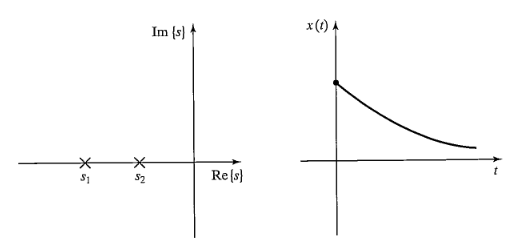
\includegraphics[width=0.5\columnwidth]{imgs/dgl_re_uneq.png}
\end{figure}

\subsubsection{Complex Roots}
\begin{itemize}
	\item If the roots are complex with negative real components → Underdamped (oscillatory decay)
	\item If the roots are complex with positive real components → Not BIBO stable (oscillatory increase)
	\item If the roots are purely imaginary → Undamped (oscillatory behavior without increase/decay)
\end{itemize}
~\\

Let $b^2 < 4mk$ \\
It follows:
$$
	x(t) = c_1e^{\lambda t}\cos(\mu t) + c_2e^{\lambda t} \sin(\mu t)
$$
, where $s_{1,2} = \lambda \pm \mu i$ \\
\\

Let $c_1 = r \cos \delta$ and \\
let $c_2 = r \sin \delta$. \\
It follows
$$
	x(t) = r e^{\lambda t} \cos(\mu t - \delta)
$$
, where \\
$r = \sqrt{c_1^2 + c_2^2}$ \\
$\delta = \atan(c_2, c_1)$

\begin{figure}[H]
	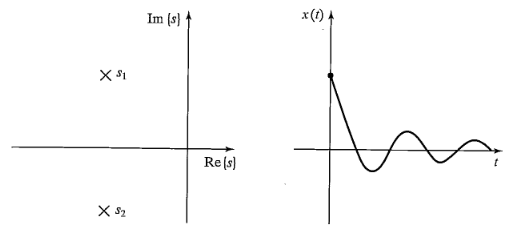
\includegraphics[width=0.5\columnwidth]{imgs/dgl_im.png}
\end{figure}

\subsubsection{Real and Equal Roots}
\begin{itemize}
	\item If the roots are real, equal and negative → Critically damped (fastest non-oscillatory exponential decay)
\end{itemize}

Let $b^2 = 4 mk$ \\
It follows:
$$
	x(t) = c_1 e^{-\frac{b}{2m}t} + c_2 t e^{-\frac{b}{2m}t}
$$

\begin{figure}[H]
	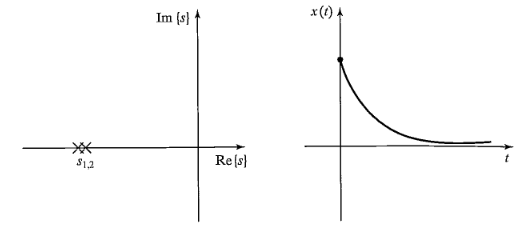
\includegraphics[width=0.5\columnwidth]{imgs/dgl_re_eq.png}
\end{figure}

\subsubsection{Damping Ratio}
Let $\zeta = \frac{b}{2\sqrt{km}}$ be the damping ratio and \\
let $\omega_n = \sqrt{k/m}$ be the natural frequency. \\
It follows:
$$
s^2 + 2\zeta \omega_n s + \omega_n^2 = 0
$$
and
\begin{itemize}
	\item $\zeta < 1$: underdamped
	\item $\zeta = 1$: critically damped
	\item $\zeta > 1$: overdamped
\end{itemize}

\subsection{Control of Second-Order Systems}
\begin{figure}[H]
	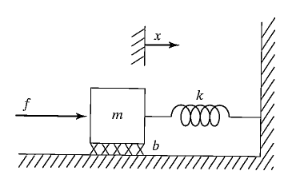
\includegraphics[width=0.5\columnwidth]{imgs/spring_mass_act.png}
\end{figure}

Let be given a spring-mass system with friction and an actuator where \\
$m$ be the mass of a block attached to the spring and \\
$k$ be the stiffness of the spring and \\
$b$ a coefficient of friction and \\
$f$ be a force applied by an actuator to the block \\
It follows:
$$
m\ddot x + b \dot x + k x = f
$$
\\

Let $x$ be the position of the block detected by a sensor and \\
let $\dot x$ be the velocity of the block detected by a sensor and \\
The force that should be applied by the actuator is computed as:
$$
	f = -k_px - k_v \dot x
$$
, where $k_p$ is the position gain and $k_v$ is the velocity gain

\subsubsection{Closed-loop Stiffness}
Let the closed-loop stiffness be $k' = k + k_p$ and \\
let $b' = b + k_v$. \\
It follows:
$$
	m\ddot x + b' \dot x + k' x = 0
$$

\begin{itemize}
	\item If $b'$ or $k'$ is negative → Unstable Control System
	\item For a critical damping: $b' = 2\sqrt{mk'}$
\end{itemize}

\subsection{Control-Law Partitioning}
\begin{itemize}
	\item Partitioning of the controller into
	\begin{itemize}
		\item a model-based portion and
		\item a servo portion
	\end{itemize}
\end{itemize}

\subsubsection{Model-based portion}
Let $f$ be the force applied by an actuator. \\
The model-based potion of the control is defined as:
$$
	f = \alpha f' + \beta
$$
, where $\alpha$ and $\beta$ are function or constants and \\
are chosen so that if $f'$ is taken as the new input to the system, the system appears to be a unit mass

\subsubsection{Model-based portion of a spring-mass system with friction}
Let be given a spring-mass system with friction and an actuator where \\
$m$ be the mass of a block attached to the spring and \\
$k$ be the stiffness of the spring and \\
$b$ a coefficient of friction and \\
$\alpha$ and $\beta$ are chosen as follows:
$$
	\alpha = m
$$
$$
	\beta = b \dot x + k x
$$
\\

For a critical damping follows: 
$$	
	k_v = 2\sqrt{k_p}
$$
, where $f' = \ddot x = -k_v \dot x - k_p x$

\begin{figure}[H]
	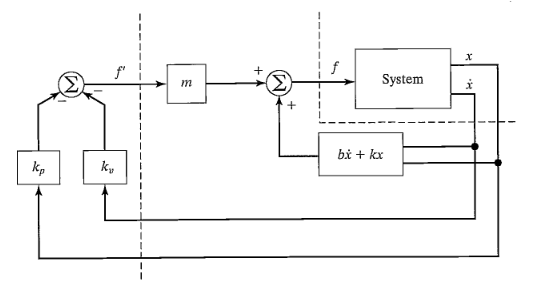
\includegraphics[width=0.5\columnwidth]{imgs/closed-loop_partitioned.png}
\end{figure}

\subsection{Trajectory-Following Control}
\subsubsection{Servo Error}
Let the trajectory be given as a function of time with\\
$x_d(t)$ be the desired position of the block and \\
$\dot x_d(t)$ be the desired velocity of the block and \\
$\ddot x_d(t)$ be the desired acceleration of the block and \\
The servo error is defined as:
$$
	e = x_d - x
$$
It follows:
$$
	\dot e = \dot x_d - \dot x
$$
and
$$
	\ddot e = \ddot x_d - \ddot x
$$

\subsubsection{Trajectory following Servo-control Law (Servo Portion)}
The servo-control law that will cause trajectory following is defined as:
$$
	f' = \ddot x_d + k_v \dot e + k_p e
$$
It follows:
$$
	\ddot e + k_v \dot e + k_p e = 0
$$


\begin{figure}[H]
	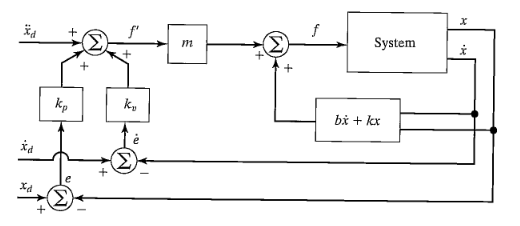
\includegraphics[width=0.5\columnwidth]{imgs/trajectory_following.png}
\end{figure}

\subsection{Disturbance Rejection}
Let $e$ be the servo error with its derivatives $\dot e$ and $\ddot e$ \\
The disturbance force is computed as:
$$
	f_{dist} = m(\ddot e + k_v \dot e + k_p e)
$$
\\

If $f_{dist}$ is bounded $\implies$ the solution of the differential equation $e(t)$ is also bounded \\
$\implies$ BIBO (bounded-input, bounded-output) stability

\subsubsection{Steady-state Error}
Let the disturbance force $f_{dist}$ be constant. \\
The steady-state error is computed as:
$$
	e = \frac{f_{dist}}{k_p}
$$
$\implies$ The higher the position gain $k_p$, the smaller will be the steady-state error.

\begin{figure}[H]
	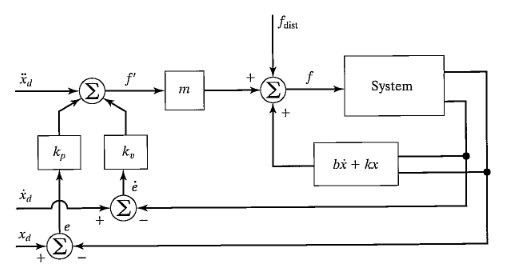
\includegraphics[width=0.5\columnwidth]{imgs/trajectory_following_fdist.png}
\end{figure}

\subsubsection{PID control law (proportional, integral, derivative control law)}
By adding an integral term to the control law to eliminate steady-state error. \\
It follows: \\
$$
	f' = \ddot x_d + k_v \dot e + k_p e + k_i \int e \textrm{ dt}
$$
\\

The disturbance force is computed as:
$$
	f_{dist} = \ddot e + k_v \dot e + k_p e + k_i \int e \textrm{ dt}
$$
If $e(t) = 0$ for $t < 0$ it follows:
$$
	\dot f_{dist} = \dddot{e} + k_v \ddot e + k_p \dot e + k_i e
$$
It follows that the steady-state error $e = 0$

%TODO proof formulas

\subsection{Continuous vs. Discrete Time Control}
\begin{itemize}
	\item Force $f$ of discussed control system is a continuous function of time, but in reality it is a discrete function of time
	\item Assumptions are valid if the computations are quickly enough
	\item Considerations in choosing a sufficiently fast sample rate:
	\begin{itemize}
		\item \textbf{Tracking reference time:} The sample rate must be at least twice the bandwidth of reference inputs
		\item \textbf{Disturbance rejection:} Sample period should be 10 times shorter than the correlation time of the noise
		\item \textbf{Antialiasing:} Sample rate should be chosen such that the amount of energy that appears in the aliased signal is small
		\item \textbf{Structural resonances:} Sample rate should be chosen at least twice the natural frequency of the resonances of mechanics
	\end{itemize}
\end{itemize}


\section{Nonlinear Control of manipulators}
\subsection{Nonlinear and Time-varying Systems}
\subsubsection{Linearization}
\begin{itemize}
	\item Make a nonlinear time-invariant system linear by using a nonlinear control term to cancel the nonlinearity in the controlled system (Linearization):
	\begin{itemize}
		\item Compute a nonlinear model-based control law that "cancels" the nonlinearities of the system to be controlled.
		\item Reduce the system to a linear system that can be controlled with the simple linear servo law developed for the unit mass.		
	\end{itemize}
\end{itemize}

\subsubsection{Control-Law Partitioning of a nonlinear system}
Let be given a spring-mass system (with friction and an actuator) with \\
a nonlinear spring relationship $f = qx^3$ and \\
the open-loop equation $m\ddot x + b \dot x + q x^3 = f$ \\
The model-based portion of the control is: 
$$
	f = \alpha f' + \beta
$$
, where
$$
	\alpha = m
$$
$$
	\beta = b \dot x + q x^3
$$
The servo portion is
$$
	f' = \ddot x_d + k_v \dot e + k_p e
$$

\begin{figure}[H]
	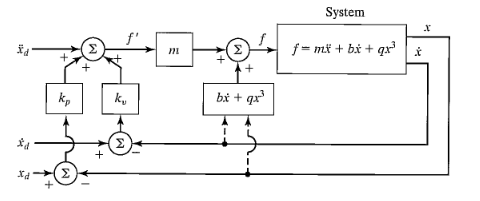
\includegraphics[width=0.5\columnwidth]{imgs/trajectory_following_nonlinear.png}
\end{figure}

\subsection{Control-Law Partitioning of a (MIMO) Multi-Input, Multi-Output Control System}
\subsubsection{Model-Based Portion}
Let $F = [f_1, \dots, f_n]^n$ be a vector of forces applied by n actuators. \\
The Model-based portion of the control is defined as: 
$$
	F = \alpha F' + \beta
$$
, where $\alpha$ is a $n \times n$ matrix and $F'$ and $\beta$ are $n \times 1$ vectors
and the model-based portion of the control law is called a linearizing and decoupling control law.

\subsubsection{Servo-Portion}
Let $E = X_d - X$ a $n \times 1$ vector of the errors in position and \\
Let $\dot E$ a $n \times 1$ vector of the errors in velocity and \\
let $X_d$ be a vector of the desired positions and \\
let $X$ be a vector of the current positions. \\
The servo law is defined as:
$$
	F' = \ddot X_d + K_v \dot E + K_p E
$$
, where $K_v$ and $K_p$ are $n \times n$ matrices, which are generally chosen to be diagonal with constant gains

\subsection{The Control Problem for Manipulators}
\subsubsection{Manipulator's Dynamic Equation with friction}
Let $\tau = M(\Theta)\ddot{\Theta} + V(\Theta, \dot{\Theta}) + G(\Theta)$ be the dynamic equation of a manipulator and \\
let $F(\Theta, \dot \Theta)$ be a model of friction dependent on the joint position $\Theta$, \\
The dynamic equation with friction is defined as:
$$
	\tau = M(\Theta)\ddot{\Theta} + V(\Theta, \dot{\Theta}) + G(\Theta) + F(\Theta, \dot \Theta)
$$

\subsubsection{Partitioning of a Dynamics Equation with Friction}
Let $\tau = M(\Theta)\ddot{\Theta} + V(\Theta, \dot{\Theta}) + G(\Theta) + F(\Theta, \dot \Theta)$ be the dynamic equation of a manipulator with friction \\
The model-based portion is defined as:
$$
	\tau = \alpha \tau' + \beta
$$
, where
$$
	\alpha = M(\Theta)
$$
$$
	\beta = V(\Theta, \dot \Theta) + G(\Theta) + F(\Theta, \dot \Theta)
$$

The servo law is defined as:
$$
	\tau' = \ddot \Theta_d + K_v \dot E + K_p E
$$
, where $E = \Theta_d - \Theta$
\\

It follows:
$$
	\ddot E + K_v \dot E + K_p E = 0
$$
and on a joint-by-joint basis:
$$
	\ddot e_i + k_{vi}\dot e + k_{pi} e = 0
$$
, where this equation is possible because the vector equation is decoupled

\begin{figure}[H]
	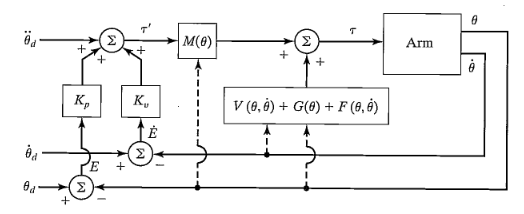
\includegraphics[width=0.5\columnwidth]{imgs/trajectory_following_dynamics.png}
\end{figure}

\subsection{Practical Considerations}
\subsubsection{Time required to compute the model}
\begin{itemize}
	\item Equations are valid if system is running in continuous time but system run in discrete time
	\item Computations in discrete time are often difficult to apply to the case of nonlinear systems
\end{itemize}

\subsubsection{Feedforward Nonlinear Control}
\begin{itemize}
	\item Place the model-based control outside the servo loop
	\item Results in: $\ddot E + M^{-1}(\Theta) K_v \dot E + M^{-1}(\Theta) K_p E = 0$
	\item Doesn't provide complete decoupling
\end{itemize}

\begin{figure}[H]
	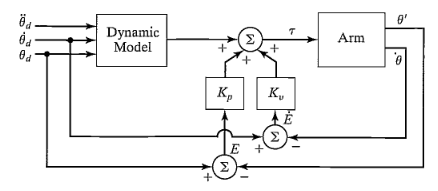
\includegraphics[width=0.5\columnwidth]{imgs/trajectory_following_feedforward.png}
\end{figure}

\subsubsection{Dual-rate computed-torque implementation}
\begin{itemize}
	\item Express the dynamic model in its configuration space form ($\tau = M(\Theta)\ddot \Theta + B(\Theta)[\dot \Theta \dot \Theta] + C(\Theta)[\dot \Theta^2] + G(\Theta)$) so that the dynamic parameters of the manipulator appear as function of manipulator position only
	\item Express the dynamic model in its configuration space form ($\tau = M(\Theta)\ddot \Theta + B(\Theta)[\dot \Theta \dot \Theta] + C(\Theta)[\dot \Theta^2] + G(\Theta)$) so that the dynamic parameters of the manipulator appear as function of manipulator position only
	\item These functions might then be computed by a background process or by a second computer or be looked up
	\item The dynamic parameters can be updated at a rate slower than the rate of the closed-loop servo
\end{itemize}

\subsubsection{Lack of knowledge of parameters}
\begin{itemize}
	\item Manipulator dynamic model often not known accurately
	\item Mass properties of objects picked up by the manipulator often not known
\end{itemize}

\subsection{Current Industrial-Robot Control Systems}
\begin{itemize}
	\item Because of problems with having good knowledge of parameters, present-day manipulators are usually controlled with very simple control laws without decoupling
	\item Most simple robot controllers do not use a model-based component at all
	\item Impossible to select fixed gains ($k_p, k_v, \dots$), instead average gain, which approximate critical damping in the center of the robot's workspace
	\item Gravity terms tend to cause static positioning errors → sometimes a gravity model is included in the control law
\end{itemize}

\subsection{Lyapunov Stability Analysis}
\begin{itemize}
	\item Applicable to linear and nonlinear systems
	\item Is concerned with determining the stability of a differential equation $\dot X = f(X)$, where $X$ is $m \times 1$ and $f(⋅)$ could be nonlinear
	\item The idea is that a positive definite ``energy-like" function of state is shown to always decrease or remain constant → the system is stable in the sense that the size of the state vector is bounded.
	\item A system is stable, if a general energy function of the system has the following properties:
	\begin{itemize}
		\item $v(X)$ has continuous first partial derivatives and $v(X) > 0$ for all X except $v(0) = 0$
		\item $\dot v(X) ≤ 0$. Here, $\dot v(X)$ means the change in $v(X)$ along all system trajectories
	\end{itemize}	
	\item If $\dot v(x) < 0$ → The system is asymptotically stable
\end{itemize}

\subsection{Cartesian-Based Control Systems}
\subsubsection{Joint-based control scheme with Cartesian-path input}
\begin{itemize}
	\item Uses the trajectory-conversion process to compute the joint trajectory from the Cartesian-based trajectory
	\item Afterwards a joint-based control scheme is used
	\item Usually just the solution for $\Theta_d$ is performed by inverse kinematics and then the joint velocities and accelerations are computed numerically by first and second differences.
\end{itemize}
\begin{figure}[H]
	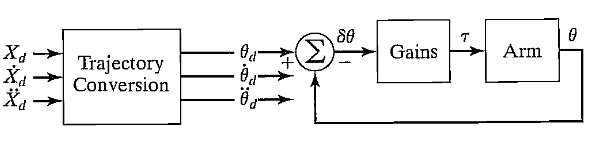
\includegraphics[width=0.5\columnwidth]{imgs/control_with_cartesian_input.png}
\end{figure}

\subsubsection{Concept of a Cartesian-based control scheme}
\begin{itemize}
	\item The sensed position of the manipulator is transformed by means of the kinematic equations into a Cartesian description of position. This Cartesian description is then compared to the desired Cartesian position in order to form errors in Cartesian space
	\item The kinematics and other transformations are now inside the loop → lower sampling frequency than joint-based control
\end{itemize}

\begin{figure}[H]
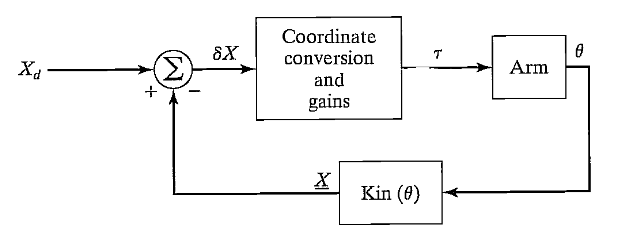
\includegraphics[width=0.5\columnwidth]{imgs/control_cartesian_basic.png}
\end{figure}

\subsubsection{Inverse-Jacobian controller} 
\textbf{Scheme:}
\begin{enumerate}
	\item Cartesian position is compared to the desired position to form an error, $\delta X$, in Cartesian space.
	\item This error may be mapped into a small displacement in joint space by means of the inverse Jacobian. 
	\item The resulting errors in joint space, $\delta \Theta$, are then multiplied by gains to compute torques that will tend to reduce these errors.
	\item The sensed position of the manipulator is transformed by means of the kinematic equations into a Cartesian description of position.
\end{enumerate}

\begin{figure}[H]
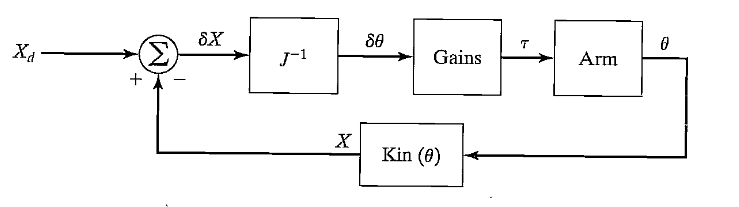
\includegraphics[width=0.5\columnwidth]{imgs/control_cartesian_inverse-jacobian.png}
\end{figure}

\subsubsection{Transpose-Jacobian controller} 
\textbf{Scheme:}
\begin{enumerate}
	\item Cartesian position is compared to the desired position to form an error, $\delta X$, in Cartesian space.
	\item This Cartesian error vector is multiplied by a gain to compute a Cartesian force vector.
	\item This Cartesian force vector (actually a force—moment vector) is then mapped through the Jacobian transpose in order to compute the equivalent joint torques that would tend to reduce the observed errors.
	\item The sensed position of the manipulator is transformed by means of the kinematic equations into a Cartesian description of position.
\end{enumerate}

\begin{figure}[H]
	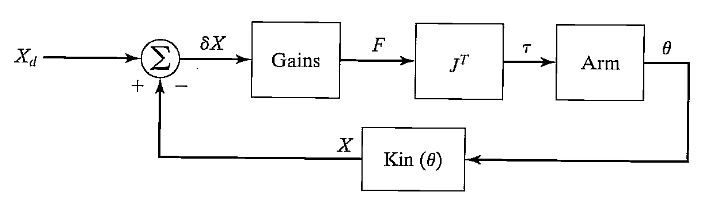
\includegraphics[width=0.5\columnwidth]{imgs/control_cartesian_transpose-jacobian.png}
\end{figure}

\subsubsection{Cartesian decoupling scheme}
\begin{itemize}
	\item Linearizing and decoupling by using $\mathcal{F} = M_X(\Theta)\ddot \chi + V_X(\Theta, \dot \Theta) + G_X(\Theta)$, where $\mathcal{F}$ is force-moment vector acting on the end-effector and $\chi$ is an Cartesian vector representing position and orientation of the end-effector
	\item Computing of the joint torques by using $\tau = \mathcal{J}^T(\Theta) \mathcal{F}$
\end{itemize}

\begin{figure}[H]
	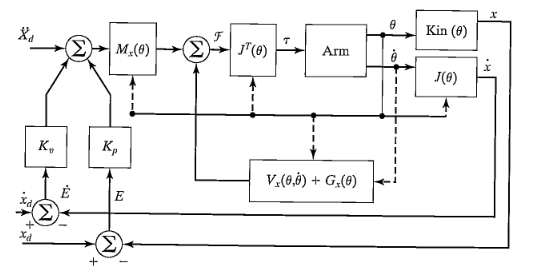
\includegraphics[width=0.5\columnwidth]{imgs/control_model-based_cartesian1.png}
\end{figure}

\begin{figure}[H]
	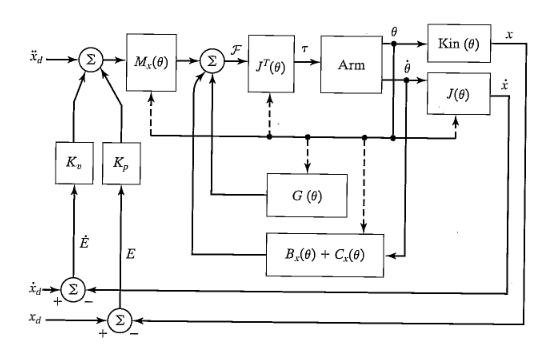
\includegraphics[width=0.5\columnwidth]{imgs/control_model-based_cartesian2.png}
\end{figure}

\subsection{Adaptive Control}
\begin{itemize}
	\item When the parameters in the model do not match the parameters of the real device, servo errors will result
	\item These servo errors could be used to drive some adaptation scheme that attempts to update the values of the model parameters until the errors disappear
\end{itemize}

\section{Force control of Manipulators}
\begin{itemize}
	\item By measuring and control contact forces generated at the hand, absolute errors in the position of the manipulator and the manipulated objects are not as important as they would be in a purely position-controlled system.
\end{itemize}
\subsection{A Framework for Control in Partially Constrained Tasks}
\begin{itemize}
	\item Tasks can be broken down into subtasks that are defined by a particular contact situation occurring between the end-effector and the work environment
\end{itemize}

\subsubsection{Natural constraints}
\begin{itemize}
	\item Constraints that result from the particular mechanical and geometric characteristics of the task configuration
	\item Natural constraint means that these constraints arise naturally from the particular contacting situation.
	\item Defined by a
	\begin{itemize}
		\item natural position (position or orientation) constraint (or often as a ``velocity equals zero" constraint) $^C\nu$ (constraint reachable positions by the environment)
		\item natural force (force or moment) constraint $^C\mathcal{F}$ (constraint forces that would cause derivative position change)
	\end{itemize}
	\item Described in terms of frame $\{C\}$, the constraint frame, which is located in the task-relevant location.
	\item $\{C\}$ could be fixed in the environment or could move with the end-effector
\end{itemize}

\subsubsection{Artificial constraint}
\begin{itemize}
	\item Introduced in accordance with the natural constraint to specify desired motions of force application.
	\item Each time the user specifies a desired trajectory in either position or force, an artificial constraint is defined.
\end{itemize}

\subsubsection{Assembly Strategy}
\begin{itemize}
	\item Term that refers to a sequence of planned artificial constraints that will cause the task to proceed in a desirable manner.
	\item Such strategies must include methods by which the system can detect a change in the contacting situation.
\end{itemize}

\subsection{The Hybrid Position/Force Control Problem}
The hybrid position/force controller must solve three problem:
\begin{itemize}
	\item Position control of a manipulator along directions in which a natural force constraint exists (due to no forces to react against).
	\item Force control of a manipulator along directions in which a natural position constraint exists. 
	\item A scheme to implement the arbitrary mixing of these modes along orthogonal degrees of freedom of an arbitrary frame $\{C\}$.
\end{itemize}

\subsection{Force Control of a Mass-Spring System}
Let be given a spring-mass system, where \\
$m$ be the mass of the block and \\
$k_e$ be the stiffness of the spring and \\
$f_{dist}$ be an unknown disturbance force. \\
The equation describing this physical system is:
$$
	f = m \ddot x + k_e x + f_{dist}
$$
or with $f_e = k_e x$
$$
	f = mk_e^{-1} \ddot f_e + f_e + f_{dist}
$$

\begin{figure}[H]
	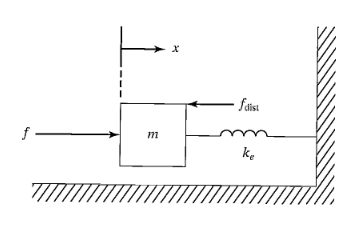
\includegraphics[width=0.5\columnwidth]{imgs/force_control_spring_mass.png}
\end{figure}


\subsubsection{Control-Law Partitioning}
\textbf{Model-based portion:} \\
Let be given a spring-mass system with the describing function $f = mk_e^{-1} \ddot f_e + f_e + f_{dist}$
The model-based portion of the control is:
$$
	f = m k_e^{-1} [\ddot f_d + k_{vf} \dot e_f + k_{pf} e_f] + f_e + f_{dist}
$$
, where
$$
	\alpha = mk_e^{-1}
$$
$$
	\beta = f_e + f_{dist}
$$
$$
	e_f = f_d - f_e
$$

\textbf{Steady-state Error:} \\
The steady-state error is computed as:
$$
	e_f = \frac{f_{dist}}{\alpha}
$$

\begin{figure}[H]
	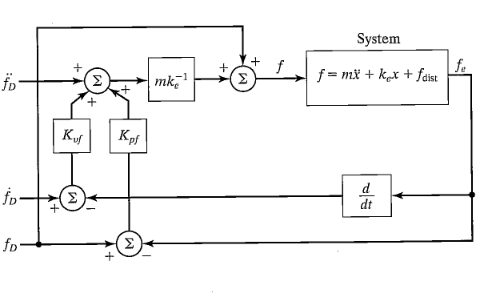
\includegraphics[width=0.5\columnwidth]{imgs/force_control_f_e.png}
\end{figure}

\textbf{Using $f_d$ instead of $f_e + f_{dist}$:} \\
The model-based portion of the control is:
$$
f = m k_e^{-1} [\ddot f_d + k_{vf} \dot e_f + k_{pf} e_f] + f_d
$$
The steady-state error is computed as:
$$
	e_f = \frac{f_{dist}}{1 + \alpha}
$$

\begin{figure}[H]
	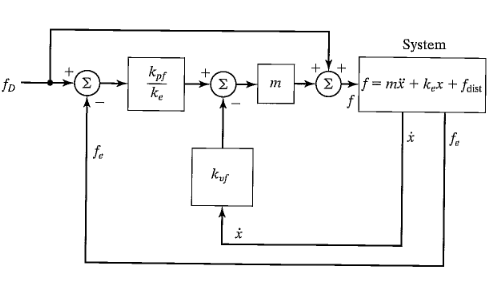
\includegraphics[width=0.5\columnwidth]{imgs/force_control_f_d.png}
\end{figure}

\subsection{The Hybrid Position/Force Control Scheme}
\subsubsection{A Cartesian manipulator aligned with \{C\}}
\begin{itemize}
	\item Let be given a 3 DOF manipulator with prismatic joints acting in the $\hat{X}, \hat{Y}$ and $\hat{Z}$ directions
	\item If we wish to be able to switch the nature of the constraint surface, we specify a complete position trajectory in all 3 DOF and a force trajectory in 3 DOF and set modes to indicate which components of which trajectory to follow.
	\item A mode uses the matrices $S$ and $S'$ to control if position or force is used to control each joint of the Cartesian arm, where $S$ and $S'$ are diagonal and a one in $S$ means, that the position control is in effect on this joint (otherwise a zero is in $S$) and a one in $S'$ means, that the force control is in effect on this joint (otherwise a zero is in $S'$).
\end{itemize}

\begin{figure}[H]
	\includegraphics[width=0.5\columnwidth]{imgs/hybrid_control_cartesian.png}
\end{figure}

E.g. $S = \begin{bmatrix}
	1 & 0 & 0 \\
	0 & 0 & 0 \\
	0 & 0 & 1
\end{bmatrix}$, 
$S' = \begin{bmatrix}
	0 & 0 & 0 \\
	0 & 1 & 0 \\
	0 & 0 & 0
\end{bmatrix}$

\subsubsection{A general manipulator}
\begin{itemize}
	\item Through use of a dynamic model written in Cartesian space, it is possible to control so that the combined system of the actual manipulator and computed model appear as a set of independent, uncoupled unit masses.
	\item For use in hybrid control scheme, the dynamics, the Jacobian and the kinematics are computed with respect to $\{C\}$.
\end{itemize}

\begin{figure}[H]
	\includegraphics[width=0.5\columnwidth]{imgs/hybrid_control_general.png}
\end{figure}

\subsection{Current Industrial-Robot Control Schemes}
\subsubsection{Passive compliance}
\begin{itemize}
	\item E.g. RCC:
	\begin{itemize}
		\item inserted between wrist and end-effector 
		\item is essentially a spring with 6 DOF
		\item Allows the end-effector to have a lower stiffness
	\end{itemize}
	\item Used in industrial applications of manipulators
\end{itemize}

%\subsubsection{Compliance through softening position gains}
%TODO








~\\\\\\
\section{Other Basics}
\subsection{Screw notation}
$\textrm{Screw}_Q(r, \phi)$ stands for the combination of a translation along an axis $Q$ by a distance $r$ and a rotation about the same axis by an angle $\phi$

\subsection{Joint axis vectors}
$$
	\hat{X} = \vect{1 \\ 0 \\ 0}
\text{,\tab}
	\hat{Y} = \vect{0 \\ 1 \\ 0}
\text{,\tab}
	\hat{Z} = \vect{0 \\ 0 \\ 1}
$$

\subsection{three-link planar arm}
A manipulator build of three parallel revolute joints is called a three-link planar arm.

\subsection{Workspace}
\begin{itemize}
	\item Volume of space that the robot end-effector of the manipulator can reach.
\end{itemize}

\subsubsection{Dextrous workspace}
\begin{itemize}
	\item Volume of space that the robot end-effector can reach with all orientations.
\end{itemize}

\subsubsection{Reachable workspace}
\begin{itemize}
	\item Volume of space that the robot can reach in at least one orientation.
\end{itemize}

\subsection{Right-Hand Coordinate System}
\begin{figure}[H]
	\includegraphics[width=0.5\columnwidth]{imgs/hand_xyz.jpg}
\end{figure}

\subsection{Schematic notation}

\subsubsection{Parallel axes}
Double hash marks on a simple schematic notation indicate that the axis are mutually parallel
\begin{figure}[H]
	\includegraphics[width=0.5\columnwidth]{imgs/3R_arm.png}
\end{figure}

\subsubsection{orthogonal axes}


\section{Mathematical Basics}
\subsection{Rotation Matrix}
\textbf{Rotation about x-axis:}
$R_x(\theta) = \begin{bmatrix}
	1 & 0 & 0 \\
	0 & \cos \theta & -\sin \theta \\
	0 & \sin \theta & \cos \theta 
\end{bmatrix}$ \\
\\

\textbf{Rotation about y-axis:}
$R_y(\theta) = \begin{bmatrix}
	\cos \theta & 0 & \sin \theta \\
	0 & 1 & 0 \\
	-\sin \theta & 0 & \cos \theta
\end{bmatrix}$ \\
\\

\textbf{Rotation about z-axis:}
$R_z(\theta) = \begin{bmatrix}
	\cos \theta & -\sin \theta & 0 \\
	\sin \theta & \cos \theta & 0 \\
	0 & 0 & 1
\end{bmatrix}$ \\
\\

\textbf{Determinant:}
$\det R = +1$

\subsection{Trigonometric Functions}

\subsubsection{Arcustangens 2}
$\atan(y,x) = \begin{cases}
	\arctan (\frac y x) & \text{if } x > 0 \\
	\arctan (\frac y x) + \pi & \text{if } x < 0 \text{ and } y > 0 \\
	\pm \pi & \text{if } x < 0 \text{ and } y = 0 \\
	\arctan (\frac y x) - \pi & \text{if } x < 0 \text{ and } y < 0 \\
	+ \frac \pi 2 & \text{if } x = 0 \text{ and } y > 0 \\
	- \frac \pi 2 & \text{if } x = 0 \text{ and } y < 0 \\
	\text{undefined} & \text{if } x = 0 \text{ and } y = 0 \\
\end{cases}$

\subsubsection{Simplifications}
$$
	\cos(\alpha + \beta) = \cos \alpha ⋅ \cos \beta - \sin \alpha ⋅ \sin \beta
$$
$$
	\sin(\alpha + \beta) = \sin \alpha ⋅ \cos \beta + \cos \alpha ⋅ \sin \beta
$$

\section{Notations}
\subsection{CoSinus}
$$
	\cos \theta_i ≡ c\theta_i ≡ c_i \text{\tab for } i \in \mathbb{N}
$$
$$
	\sin \theta_i ≡ s\theta_i ≡ s_i \text{\tab for } i \in \mathbb{N}
$$

\subsection{CoSinus2}
$$
	c_{12} = c_1c_2 - s_1s_2 = \cos(\theta_1 + \theta_2)
$$
$$
	s_{12} = c_1s_2 + s_1c_2 = \sin(\theta_1 + \theta_2)
$$

\subsection{CoSinus3}
$$
	c_{123} = c_1s_2s_3 + s_1s_2c_3 - s_1c_2s_3 - c_2c_3c_4
$$
$$
	s_{123} = s_1c_2c_3 + c_1c_2s_3 - c_1s_2c_3 - s_1s_2s_3
$$

\pagebreak
\section*{Note}
This is a summary of the lecture Robotics of the Technical University Munich.
This lecture was presented by Burschka D. in the winter semester 2018/19.
This summary was created by Gaida B.
All provided information is without guarantee.

\section*{References}
John J. Craig. \textit{Introduction to Robotics Mechanics and Control}. Pearson Education, Inc. New York. 2005

\end{document}








